%!TEX root = main.tex

\section{Simulations} % (fold)
\label{sec:simulations}

\subsection{Initial Trials with Sinusoidal Waves} % (fold)
\label{ssub:initial_trials_with_sinusoidal_waves}
The simplest, and so easiest to program, wave is the sine wave. Figure~\ref{fig:initialsines} shows two examples of a sine wave that is created at the centre of the simulation region. The boundaries are currently totally reflecting and so the waves are reflected back towards the centre where they interfere with each other. The boundaries can be set to absorbing, in which case the wave moves through them and disappears. This has the same appearance as if there were no boundaries and the wave continued to infinity. The relative difference between the magnetic and electric fields is set to a half so that they both can be easily distinguished.
\begin{figure}[ht]
        \centering
        \begin{subfigure}[ht]{0.45\textwidth}
                \centering
                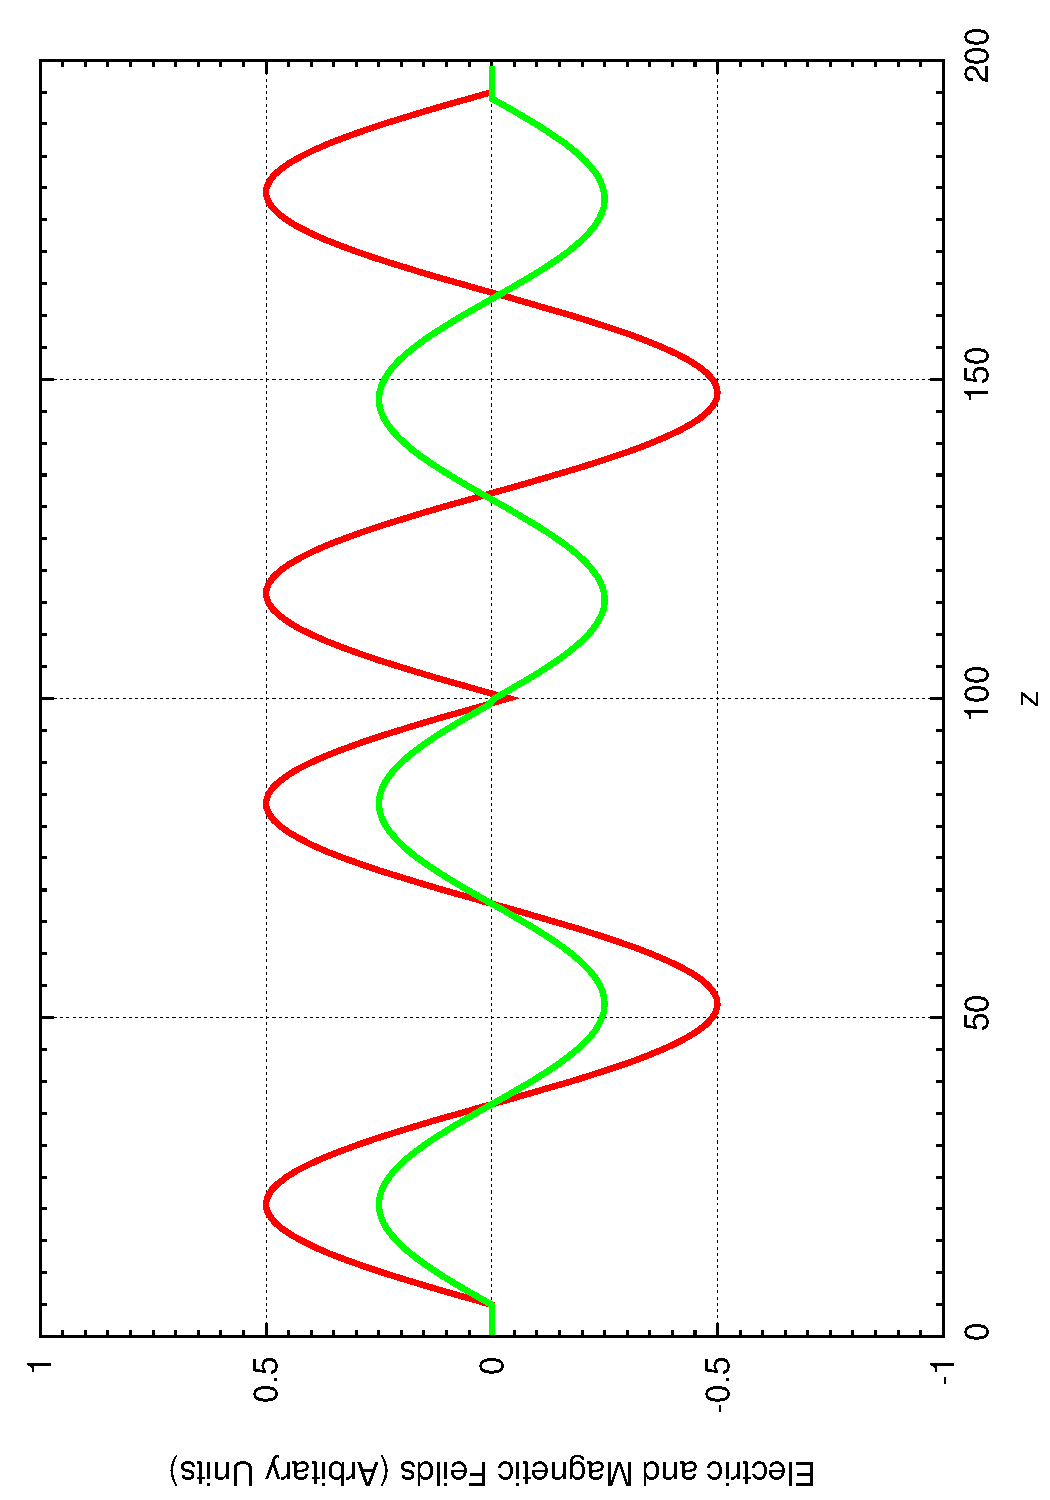
\includegraphics[angle=270, width=\textwidth]{infsine.pdf}
        \end{subfigure}%
        ~
        \begin{subfigure}[ht]{0.45\textwidth}
                \centering
                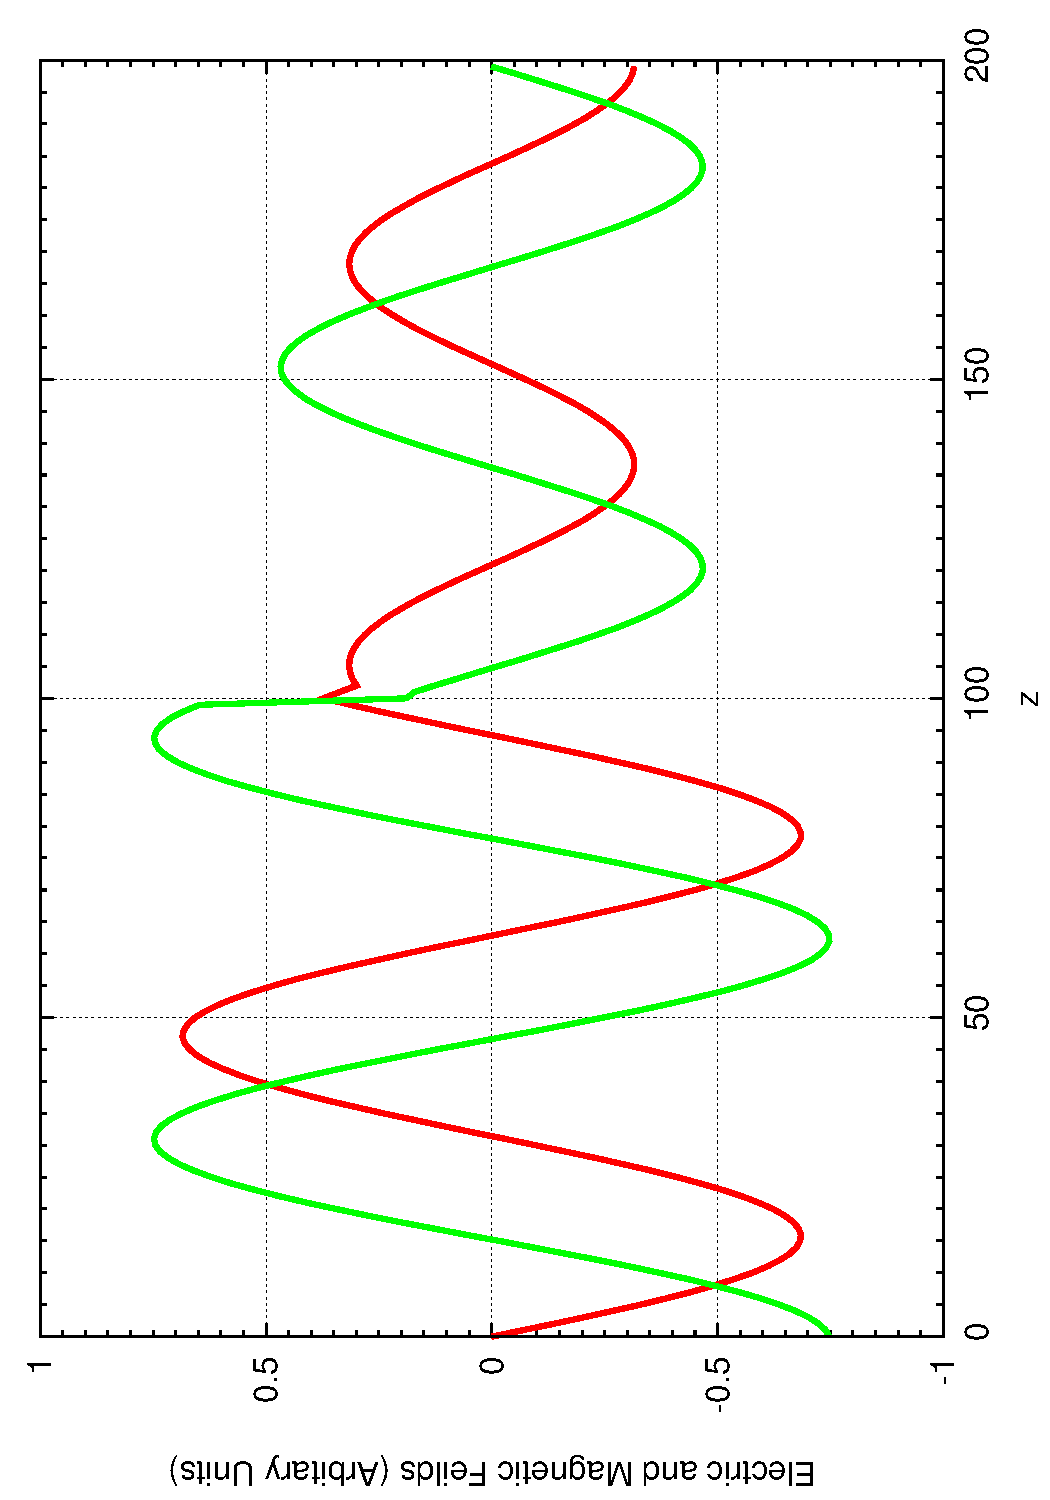
\includegraphics[angle=270, width=\textwidth]{boundsine.pdf}
        \end{subfigure}
        \caption{Two frames from a sine wave that is created in the centre of the region. The first wave is a simple sine wave in a system with perfectly absorbing boundaries. The seconds shows the same sine wave, but with reflecting boundaries and given more time to evolve.}\label{fig:initialsines}
\end{figure}

Since the source is continually creating the wave, the amplitude of the waves in the bounded case increases as the existing reflected waves interfere with the newly created ones. 
% subsubsection initial_trials_with_sinusoidal_waves (end)

\subsection{Initial Trials with Gaussian Pulse} % (fold)
\label{sub:initial_trials_with_gaussian_pulse}
A slightly more complex function is the Gaussian function that generates a pulse of a specified width and height. This function has the equation
\begin{align}
        f(x) &= a\cdot\e{-\frac{(x-b)^2}{2c^2}} \label{eq:gaussian}
\end{align}
where $a$, $b$ and $c$ are constants that determine the width, height and position of the function.

Three frames showing the start of the wave are shown in figure~\ref{fig:initialguass}. This time the wave is created at the origin, again the boundaries are totally absorbing. A point to note is that, though in this case, the magnetics field, green, is negative and the electric field, red, is positive, these relations really have no physical meaning. This representation is used so that the relative position of the two waves can be seen. In reality, the two components of the wave will be at $90^{\circ}$ to each other so that one is in the $x$-axis and the other in the $y$-axis. The relative signs of the wave with respect to the other depends on the direction of travel, as defined by the ``right hand rule''. Later, the wave is represented in three dimensions where the relation between the two is more physically accurate.
\begin{figure}[ht]
        \centering
        \begin{subfigure}[ht]{0.45\textwidth}
                \centering
                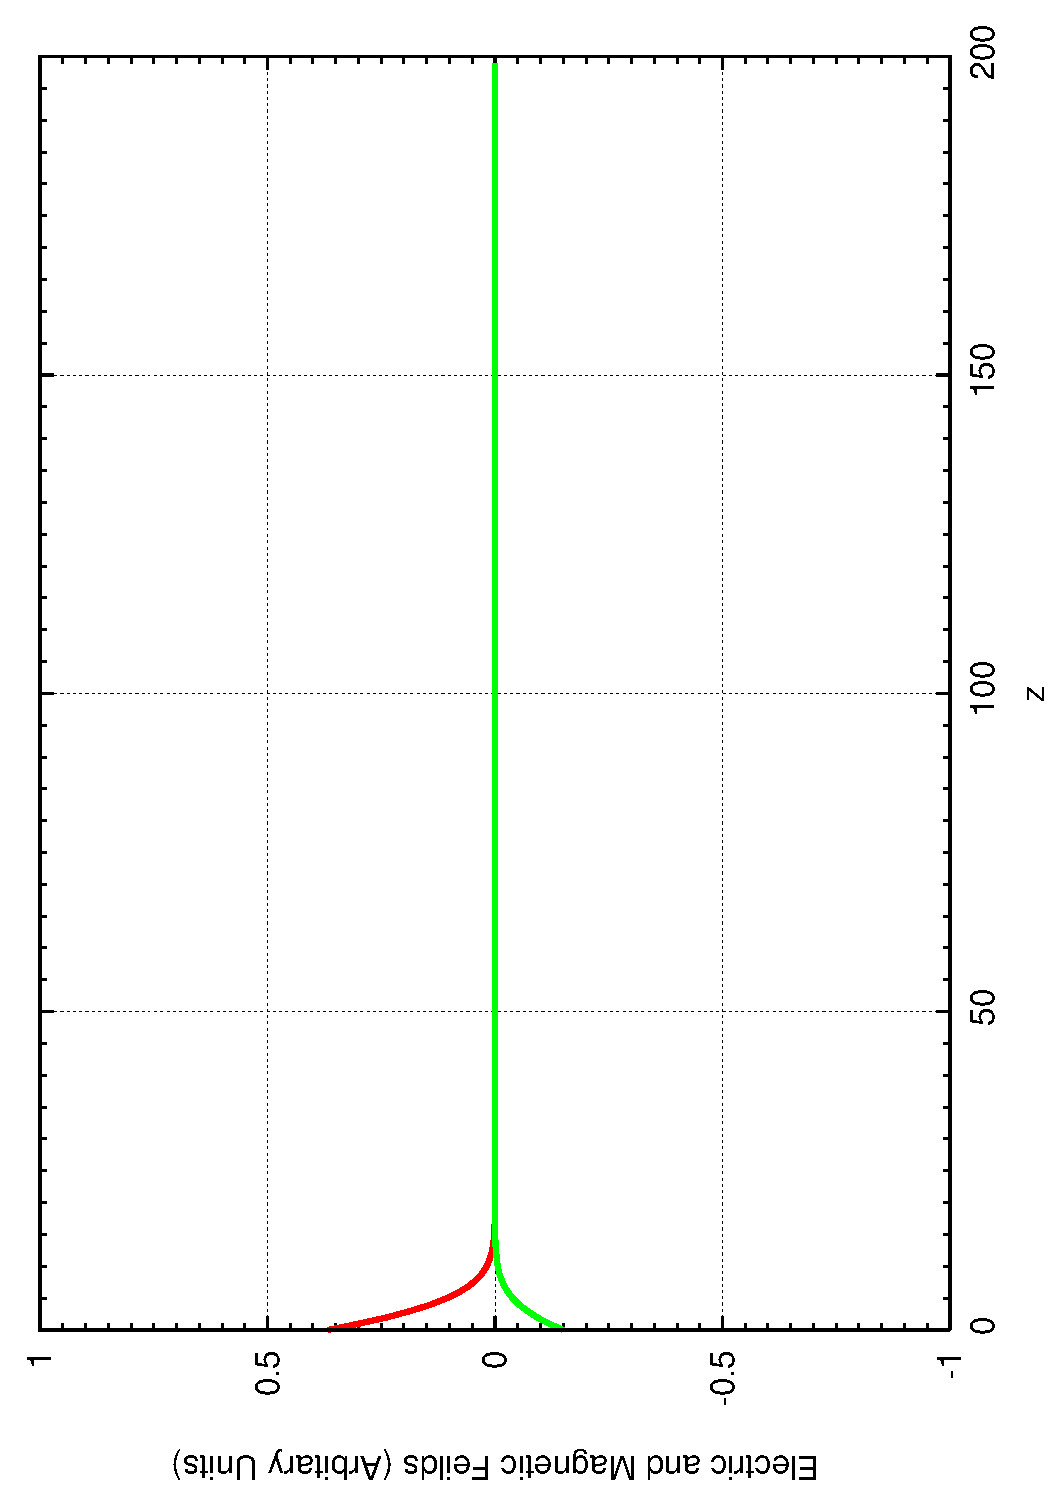
\includegraphics[angle=270, width=\textwidth]{initialguass1.pdf}
        \end{subfigure}%
        ~
        \begin{subfigure}[ht]{0.45\textwidth}
                \centering
                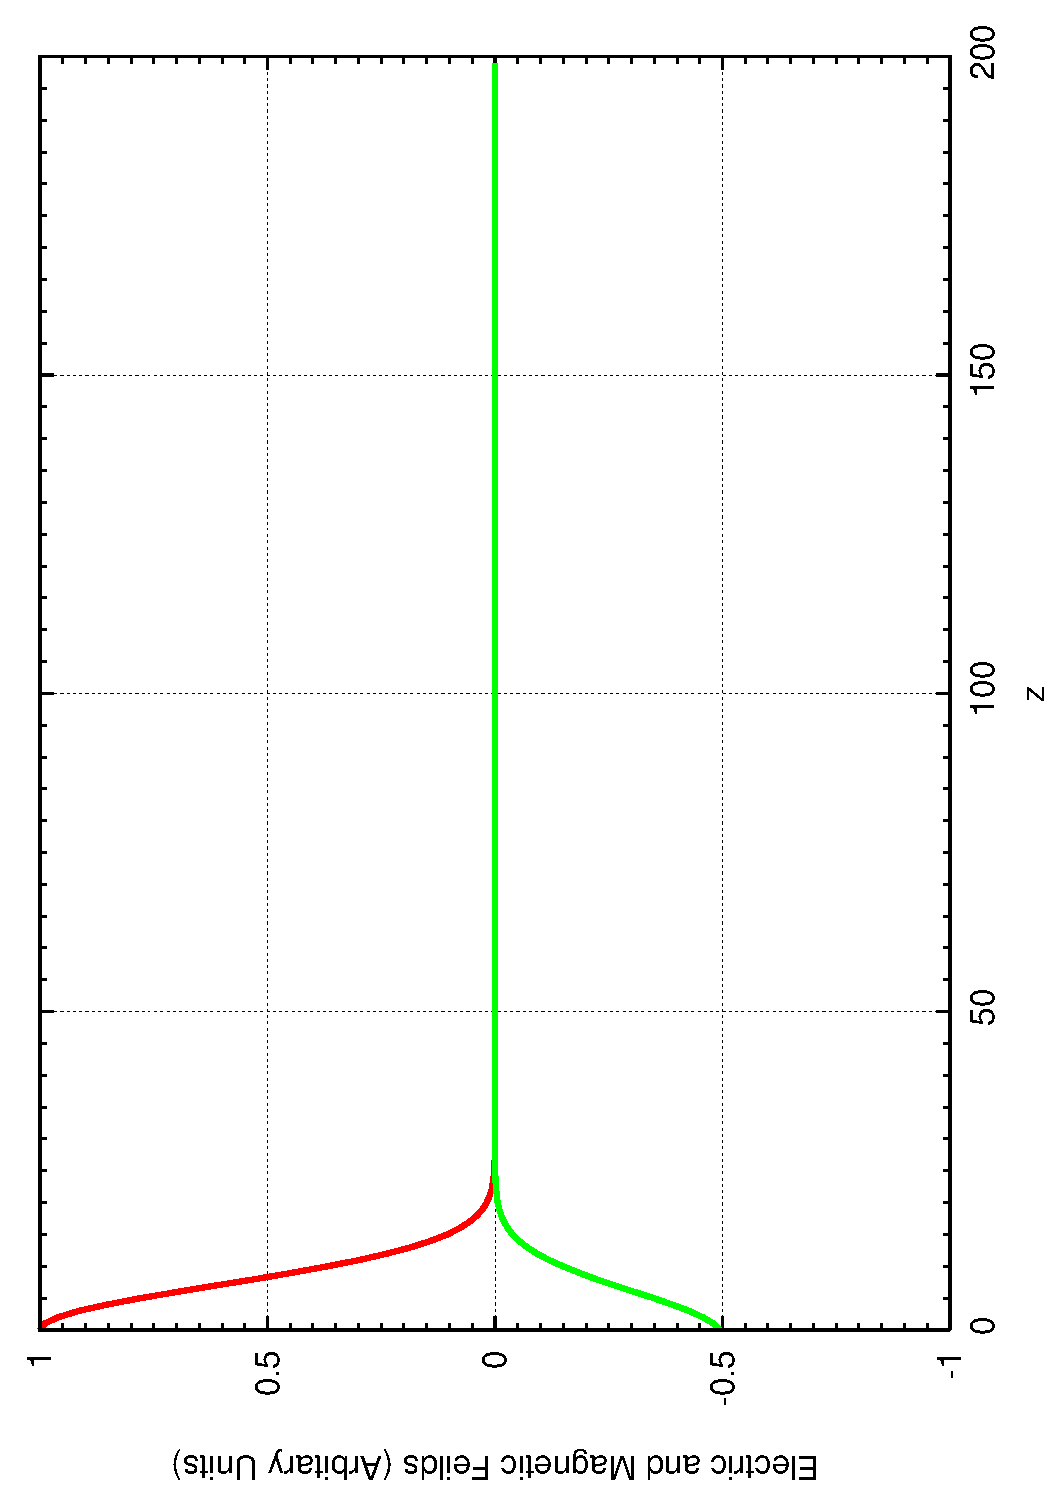
\includegraphics[angle=270, width=\textwidth]{initialguass2.pdf}
        \end{subfigure}

        \begin{subfigure}[ht]{0.45\textwidth}
                \centering
                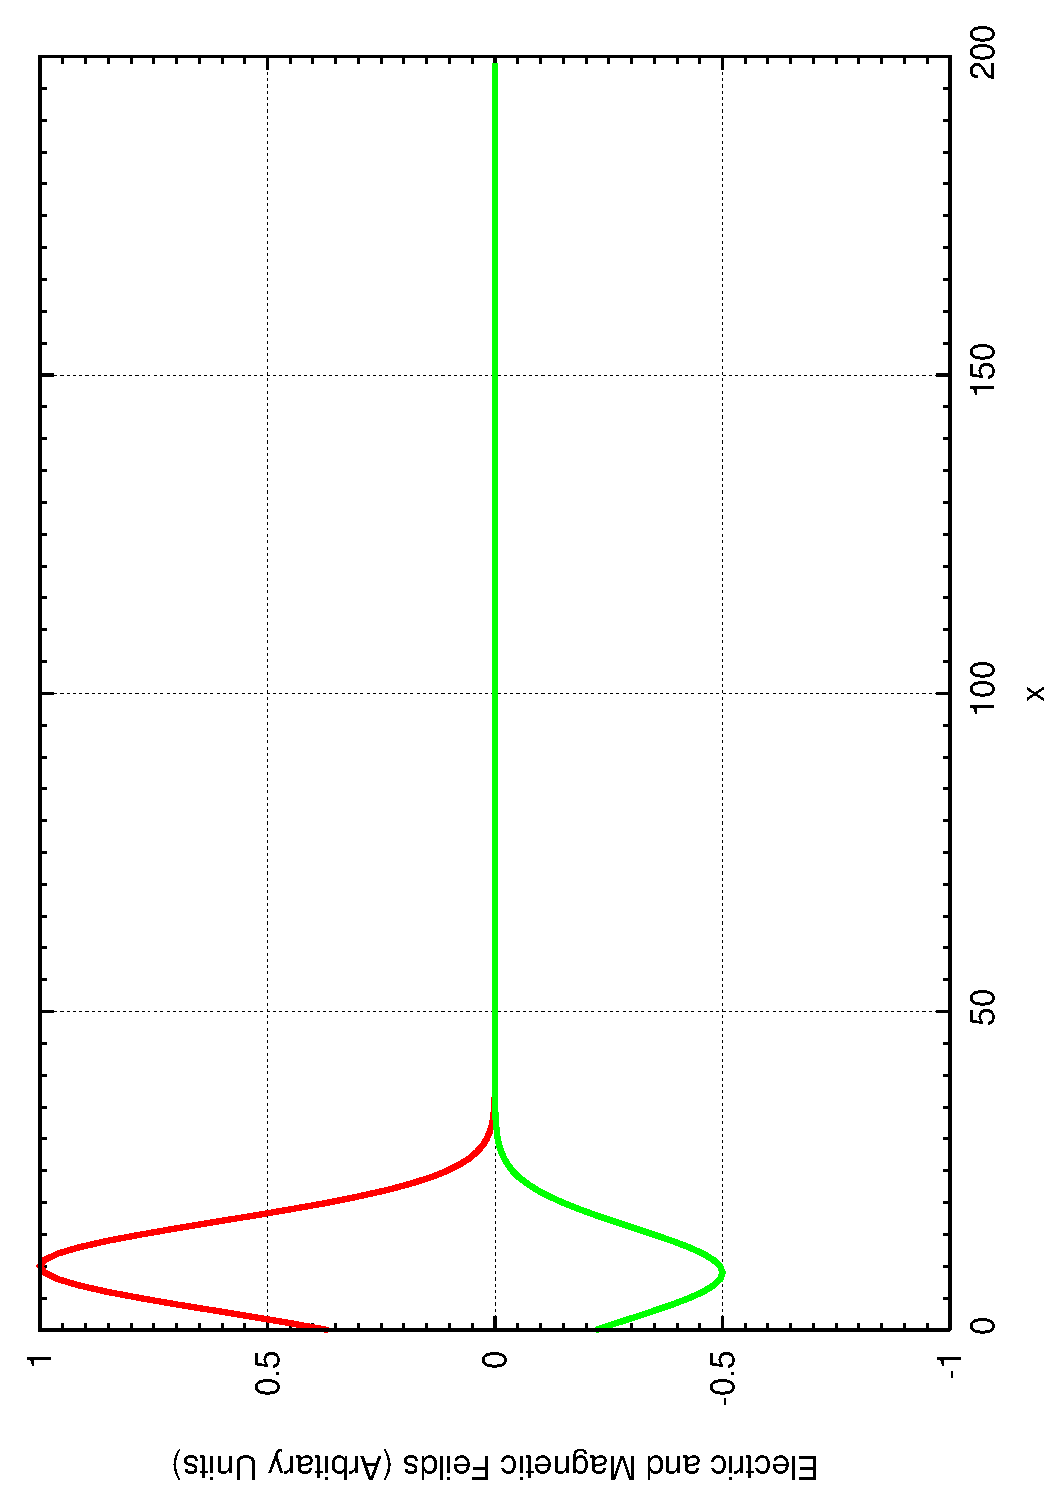
\includegraphics[angle=270, width=\textwidth]{initialguass3.pdf}
        \end{subfigure}
        ~
        \begin{subfigure}[ht]{0.45\textwidth}
                \centering
                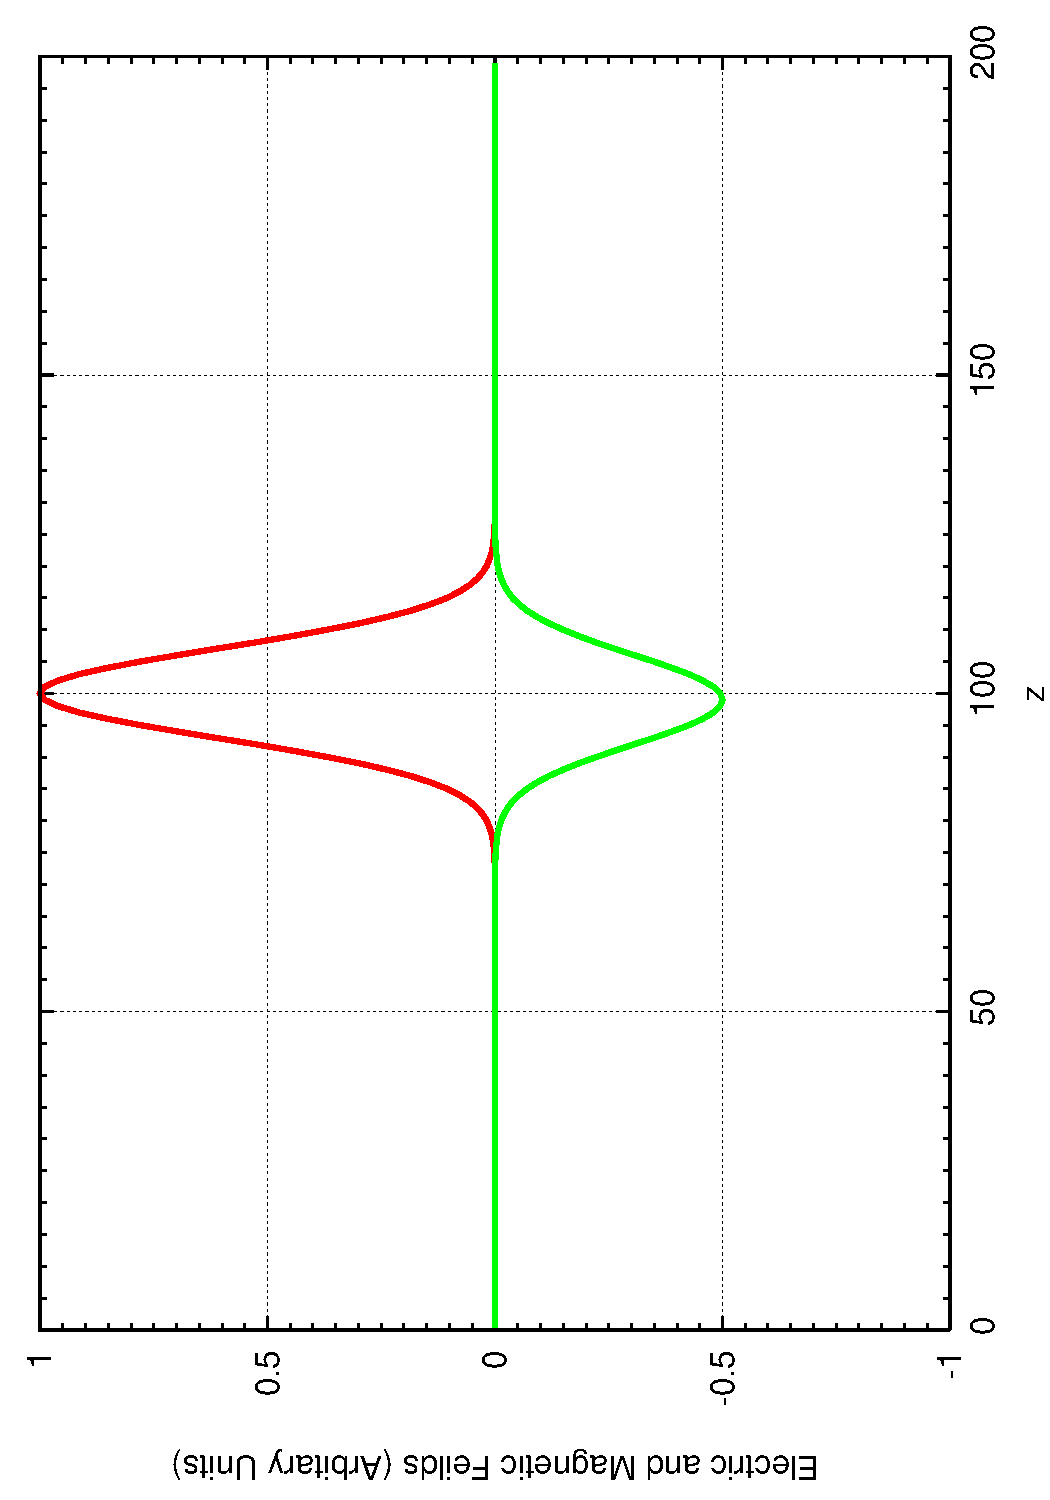
\includegraphics[angle=270, width=\textwidth]{initialguass4.pdf}
        \end{subfigure}
        \caption{An image of three frames each 10 frames apart showing the development and the start of propagation of a Gaussian shaped pulse, as well as a frame showing the pulse as it traverses the simulation area.}\label{fig:initialguass}
\end{figure}

This wave can be seeded at any point in the $z$ axis within the simulation area, $[0,200]$, as specified by the user. If the starting point for the wave is within the area, as opposed to at either edge, then two waves are generated and propagate in both directions away from the centre, figure~\ref{fig:initialcenter}.
\begin{figure}[ht]
        \centering
        \begin{subfigure}[ht]{0.45\textwidth}
                \centering
                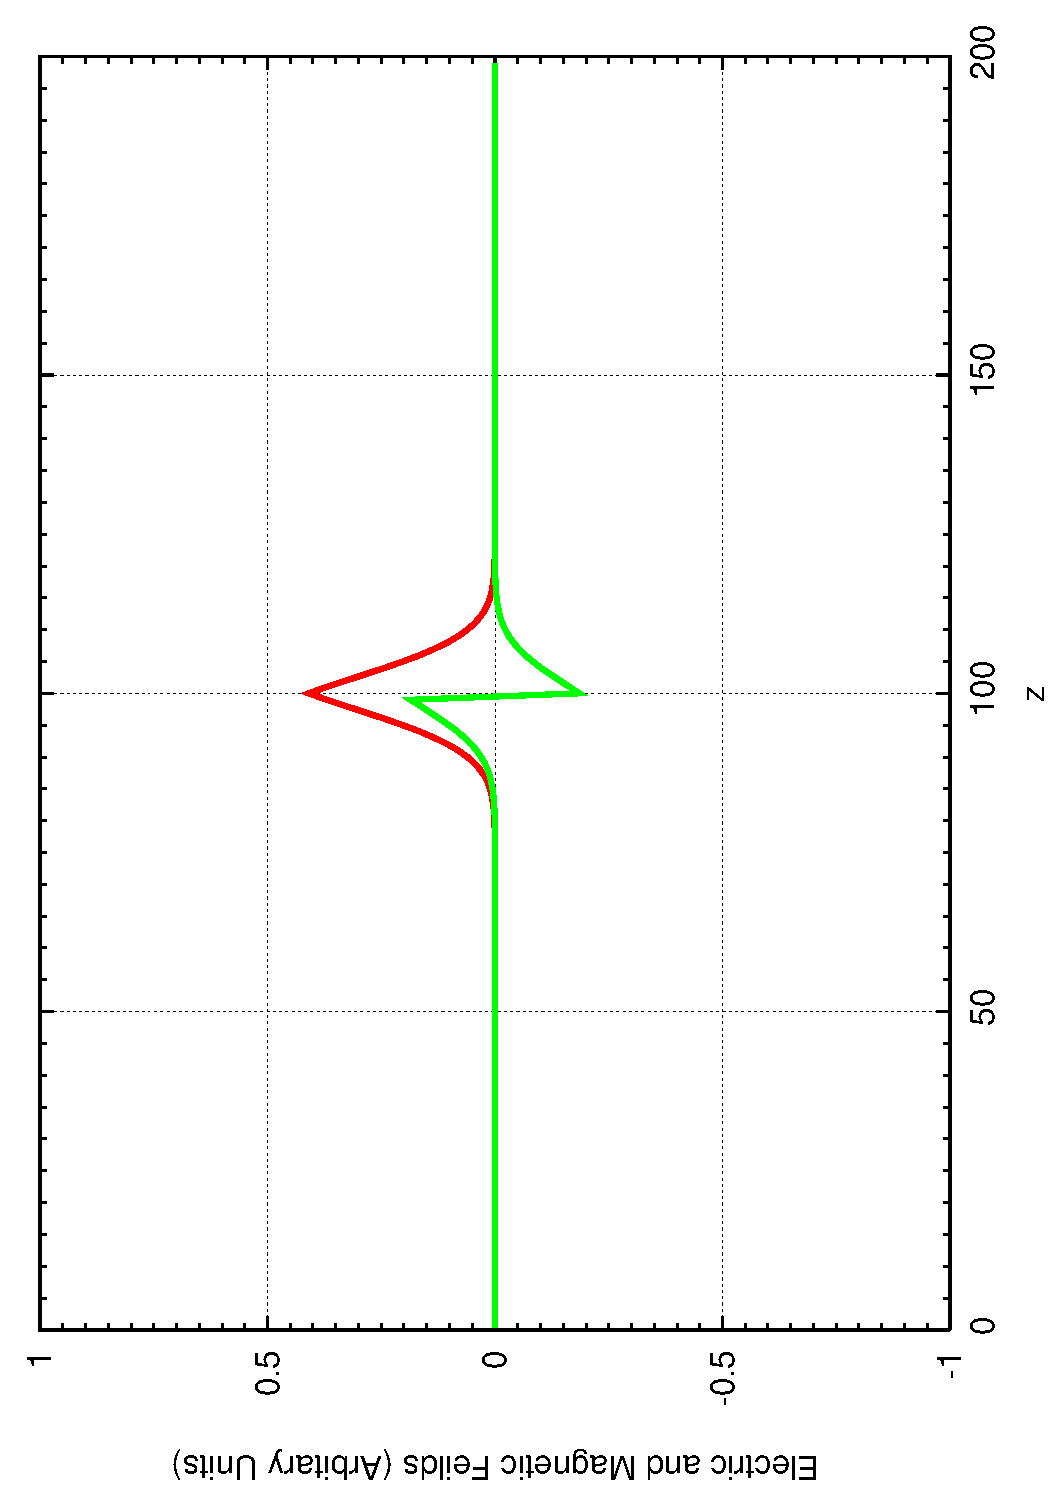
\includegraphics[angle=270, width=\textwidth]{centerseed1.pdf}
        \end{subfigure}%
        ~
        \begin{subfigure}[ht]{0.45\textwidth}
                \centering
                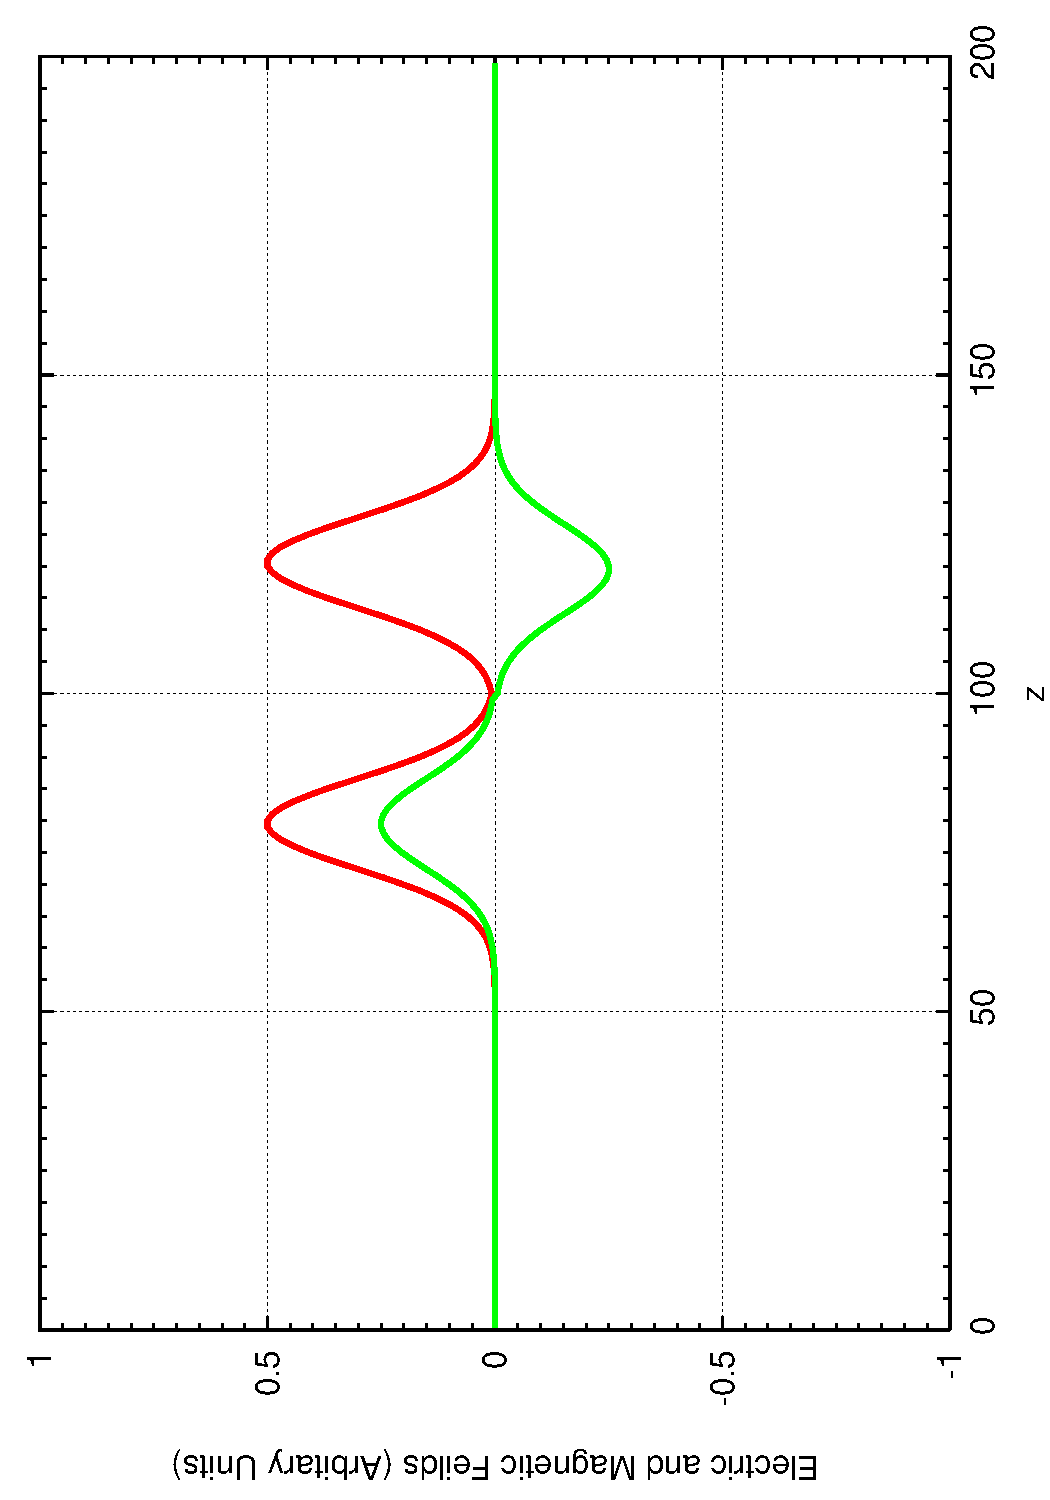
\includegraphics[angle=270, width=\textwidth]{centerseed2.pdf}
        \end{subfigure}
        \caption{Two frames from a wave that is created in the centre of the region. The seed point creates two pulses that move away from each other. The amplitude is set to one half of previous so that when they interact after colliding with the walls, the resulting peak stays within the graphing area.}\label{fig:initialcenter}
\end{figure}

Figure~\ref{fig:initialcenter} shows clearly the difference in the sign of the magnetic wave, which is calculated from the electric, when moving in opposite directions. The discontinuity in the magnetic wave in the first image is due to the discontinuity of the first derivative of the electric wave when it is created. 
% subsection initial_trials_with_gaussian_pulse (end)

\subsection{Dielectric Material} % (fold)
\label{sub:dielectirc_material}
A dielectric material is an electrical insulator that can be polarized by an electric field. This means that when an electric field enters a dielectric material, some of the energy is lost to the material and so the amplitude of the wave decreases. 

\subsubsection{Non-Lossy Material} % (fold)
\label{ssub:non_lossy_material}
We shall first consider the case where a dielectric medium is placed in the simulation area which has a finite, non-zero permittivity, but is not lossy. This means that the material will cause an incident wave to be partly transmitted, but also partly reflected. 

The absolute permittivity of a dielectric material is a measure of the resistance felt when forming an electric field inside a conducting material. It is given by equation~\ref{eq:absepsilon}.
\begin{align}
    \epsilon &= \epsilon_r \epsilon_0 \label{eq:absepsilon}
\end{align}
where $\epsilon_0=8.85419\times 10^{-12}\,\text{Fm}^{-1}$ is the permittivity of free space and $\epsilon_r$ is the relative permittivity of the material in question. It is this value that shall be changed for the dielectric in the simulation. A value of $\epsilon_r=10.0$ is used in the simulation which is roughly comparable to that of graphite or salt (NaCl). 

If a dielectric is placed in the simulation area, the wave will be incident on it and decrease in amplitude as it travels trough. In order to conserve the energy and momentum of the wave, part of the wave is reflected back from the boundary between free space and the dielectric. The ratio of the transmitted wave to the reflected wave is given by equation~\ref{eq:reflectioncoeff}.
\begin{align}
    C &= \frac{R}{T}, \label{eq:reflectioncoeff}
\end{align}
where $C$ is the reflection coefficient of the reflected wave of amplitude $R$, which is produced when an initial wave hits a boundary, and the transmitted wave with amplitude $T$, which travels through the boundary. This is equal to 
\begin{align}
    C &= \left| \frac{n_1\cos\theta_i - n_2\cos\theta_t}{n_1\cos\theta_i + n_2\cos\theta_t}\right|^2 
    \intertext{Using Snell's law, $\frac{\sin\theta_i}{\sin\theta_t} = \frac{n_2}{n_1}$, this can be written as}
    C &= \left| \frac{n_1\cos\theta_i - n_2\sqrt{1-\left( \frac{n_1}{n_2}\sin\theta_i \right)^2}}{n_1\cos\theta_i + n_2\sqrt{1-\left( \frac{n_1}{n_2}\sin\theta_i \right)^2}} \right|^2
    \intertext{Since, in this situation, the waves are approaching the boundary at $90^\circ$, this reduces to}
    C &= \left| \frac{n_1 - n_2}{n_1 + n_2} \right|^2
\end{align}

An example, again using the Gaussian function, can be seen in figure~\ref{fig:dielectricgauss}. Here, free space is represented by a white background and the dielectric is the grey shaded area.
\begin{figure}[ht]
        \centering
        \begin{subfigure}[ht]{0.45\textwidth}
                \centering
                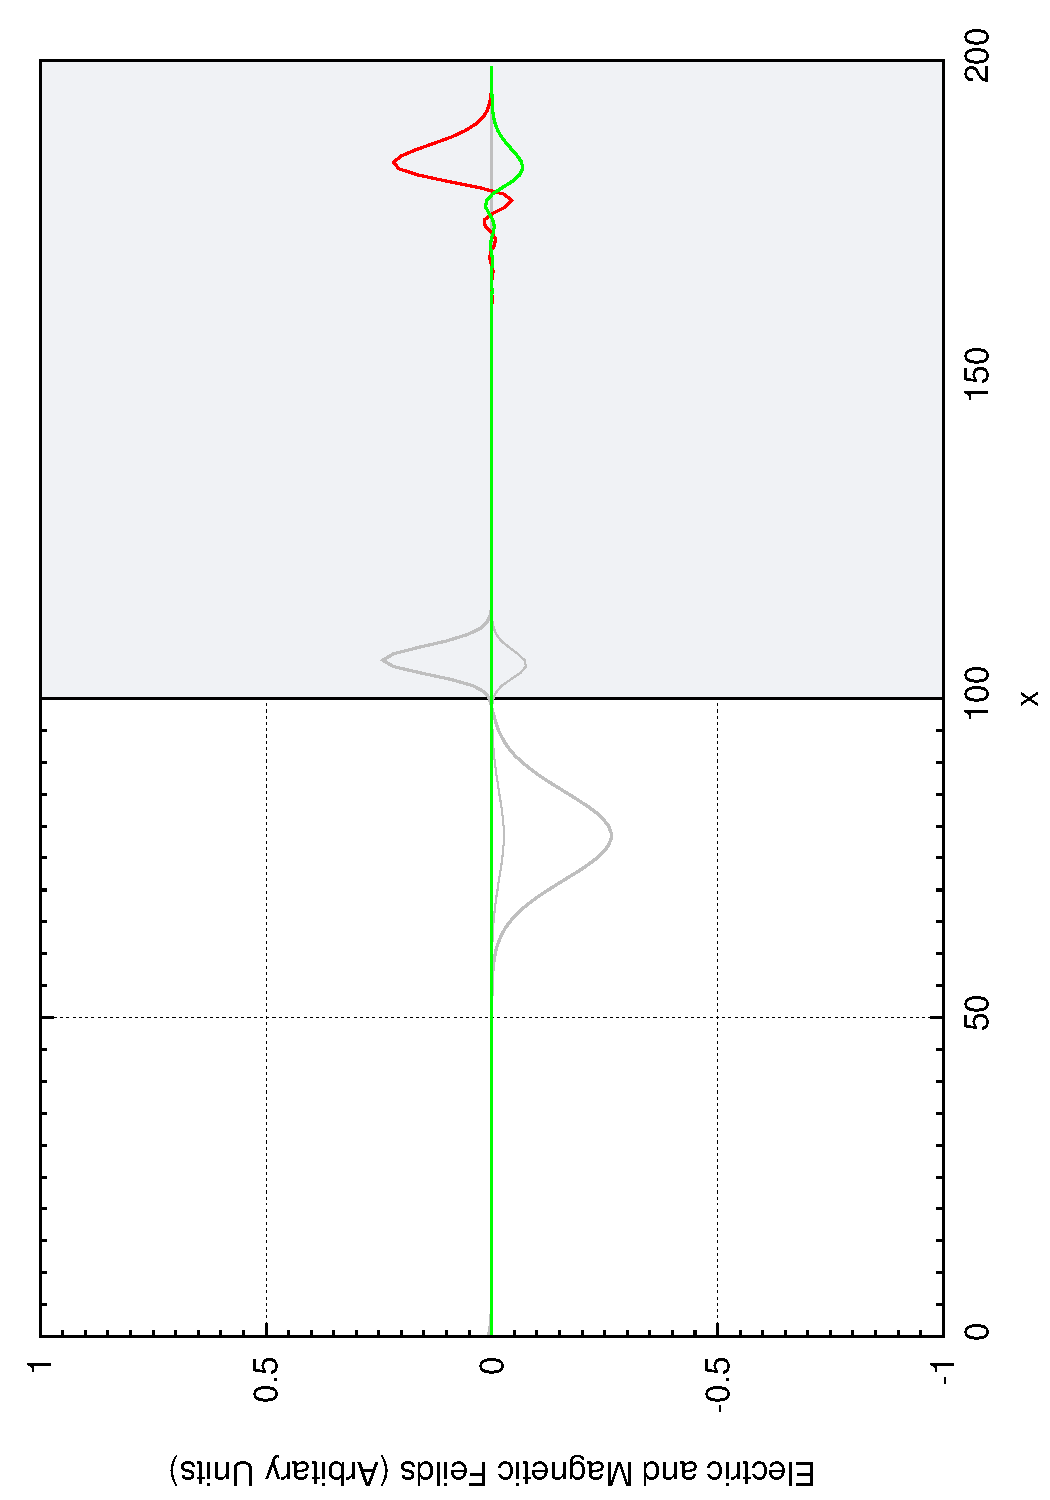
\includegraphics[angle=270, width=\textwidth]{dielectricdouble.pdf}
        \end{subfigure}%
        ~
        \begin{subfigure}[ht]{0.45\textwidth}
                \centering
                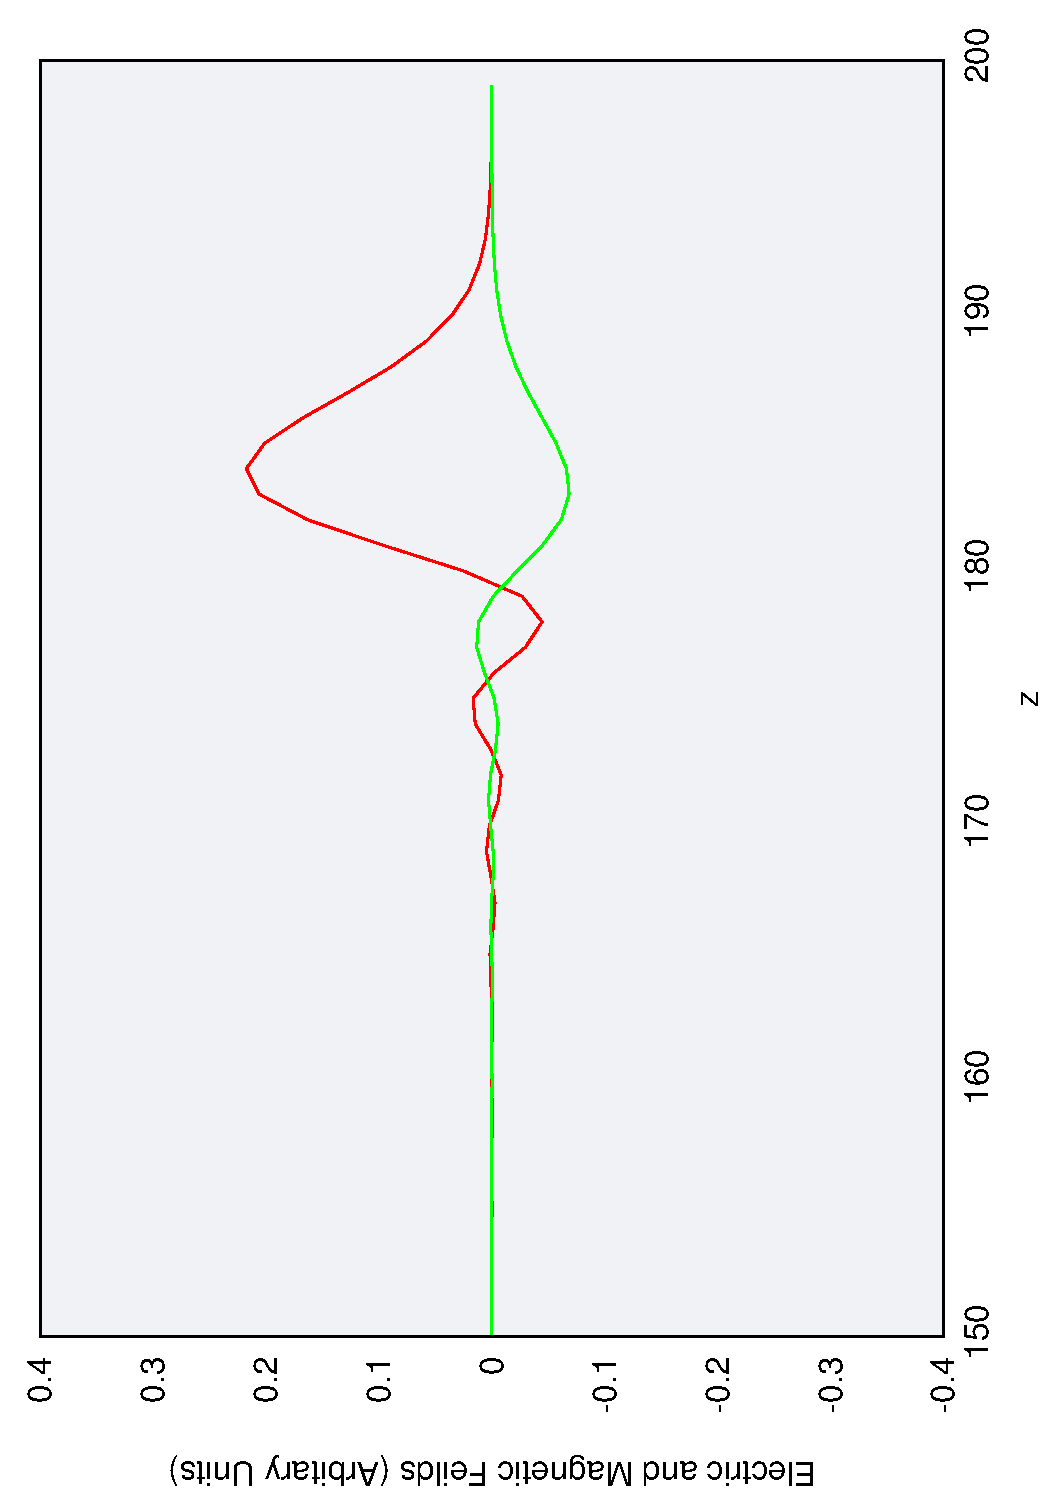
\includegraphics[angle=270, width=\textwidth]{gaussnoise1b.pdf}
        \end{subfigure}
        \caption{A dielectric is now added to the simulation area. This dielectric is not lossy , so the propagating wave does not loose any energy, but it has a finite permittivity of 10 so that the amplitude is decreased when the wave is incident on the dielectric boundary. Part of the wave is reflected back and some propagates through the material. The first image shows the wave just after it has hit the boundary where a reflected and transmitted wave of equal magnitude but opposite sign and different width are seen. And the second image shows a larger image of the transmitted wave as it propagates through the medium. The departure from a true Gaussian function can be seen clearly here as well as the limitation of the simulation in the straight lines that make up the curve.}\label{fig:dielectricgauss}
\end{figure}

The second diagram in figure~\ref{fig:dielectricgauss} shows the wave once it has propagated a significant distance through the dielectric material. This wave resembles a sinusoidal pulse instead of the simple Gaussian function since there are extra periods to the function behind the main peak. These smaller peaks are not physical and are instead an artefact of computation.

These peaks are due to the temporal/spacial time step of the simulation being relatively large. This can be demonstrated by increasing the frequency of a sine wave, while keeping other factors constant. Figure~\ref{fig:highfreqsine} shows a series of sine wave with increasing frequency.
\begin{figure}[ht]
        \centering
        \begin{subfigure}[ht]{0.45\textwidth}
                \centering
                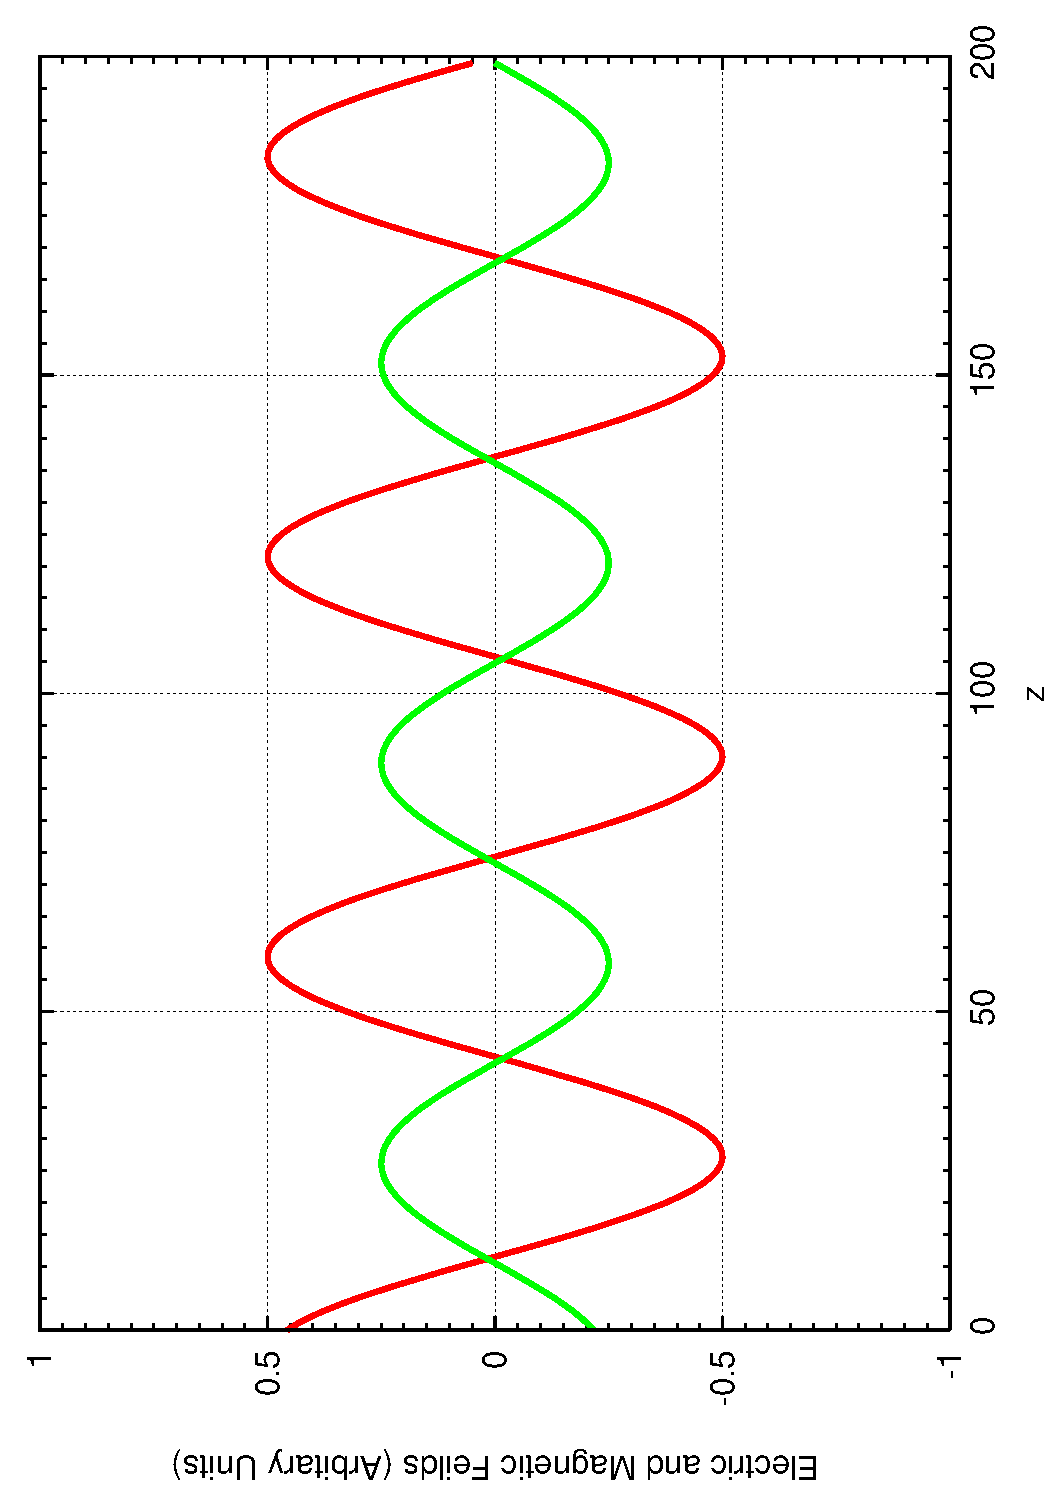
\includegraphics[angle=270, width=\textwidth]{highfreqsine1.pdf}
        \end{subfigure}%
        ~
        \begin{subfigure}[ht]{0.45\textwidth}
                \centering
                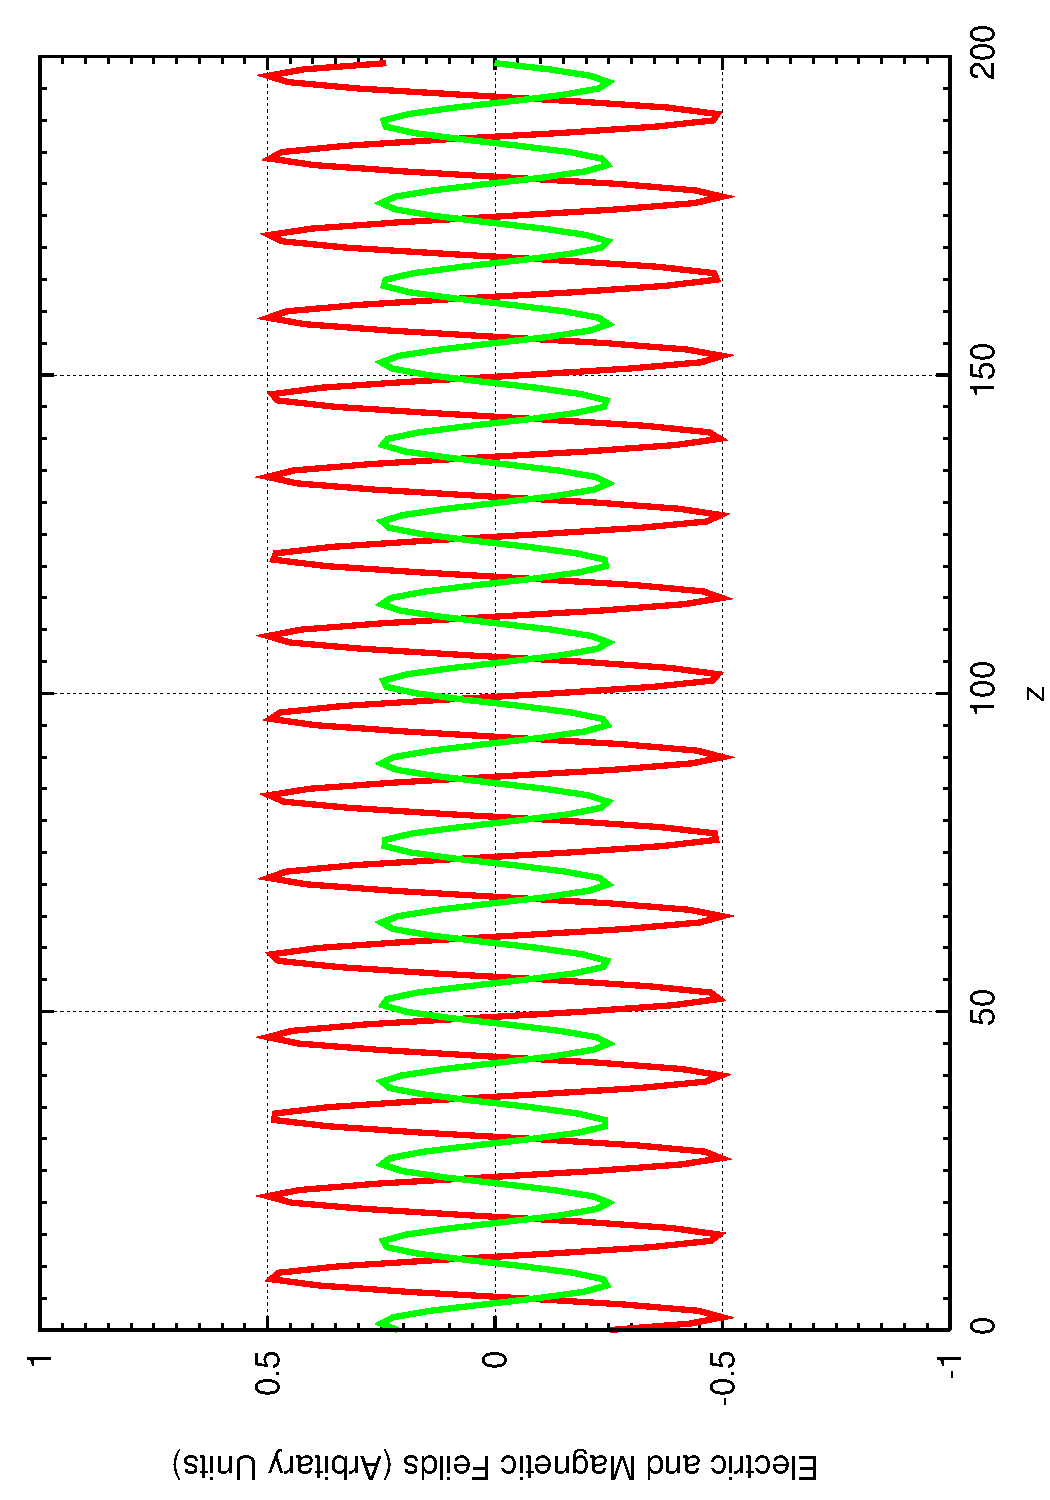
\includegraphics[angle=270, width=\textwidth]{highfreqsine2.pdf}
        \end{subfigure}

        \begin{subfigure}[ht]{0.45\textwidth}
                \centering
                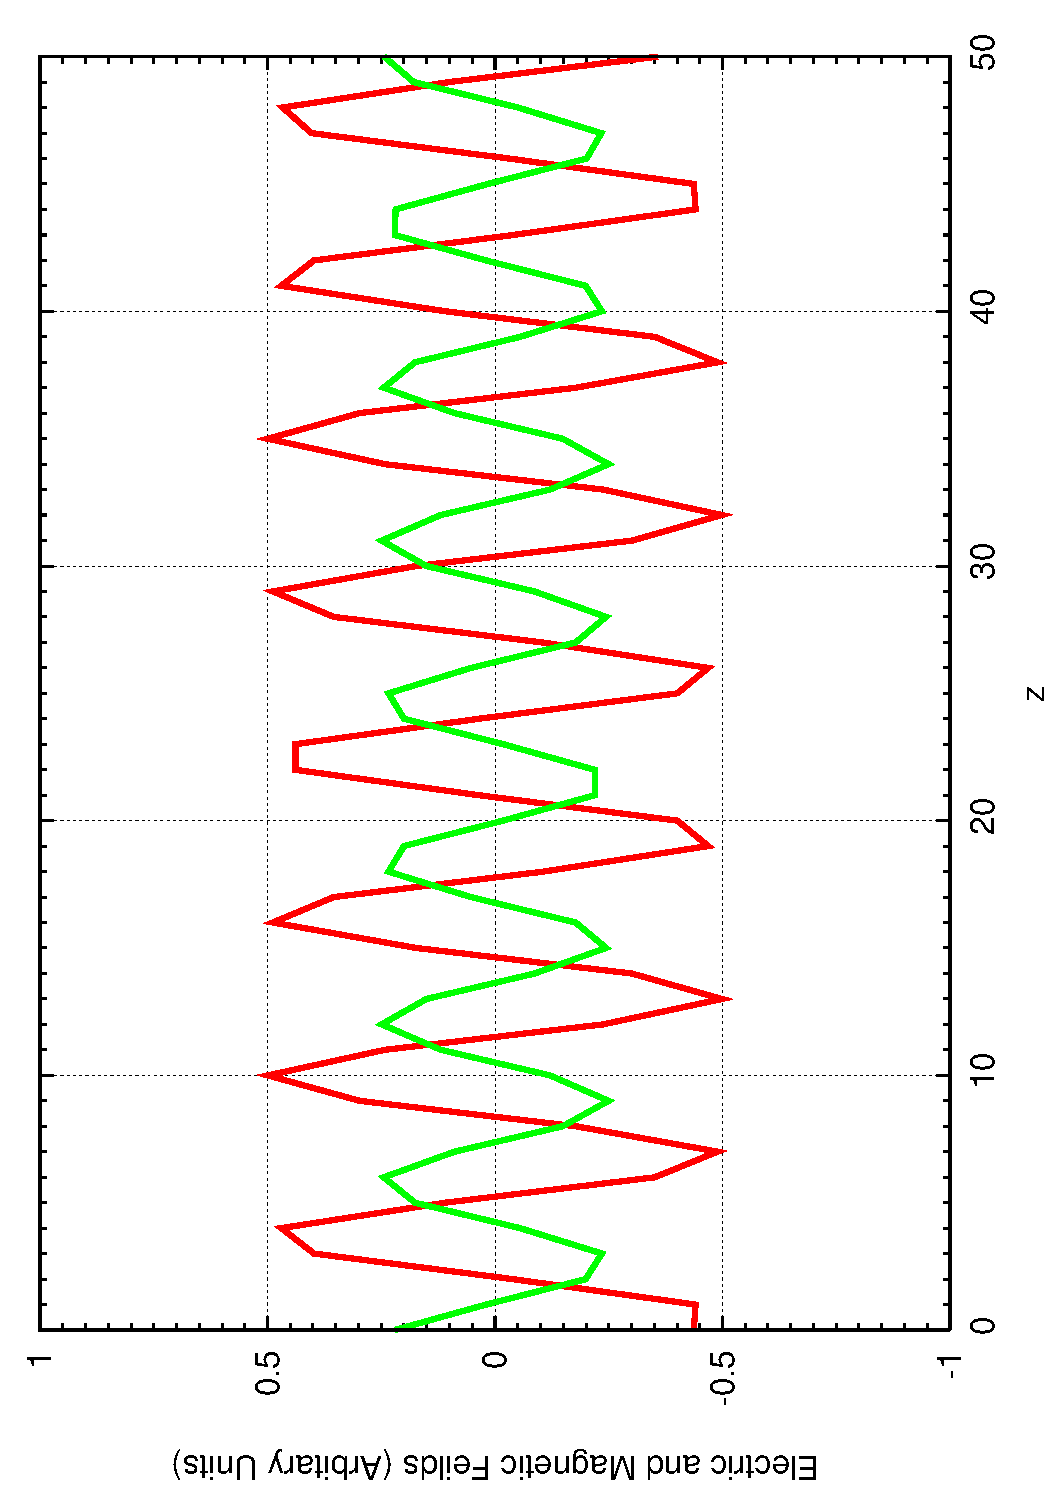
\includegraphics[angle=270, width=\textwidth]{highfreqsine3.pdf}
        \end{subfigure}
        ~
        \begin{subfigure}[ht]{0.45\textwidth}
                \centering
                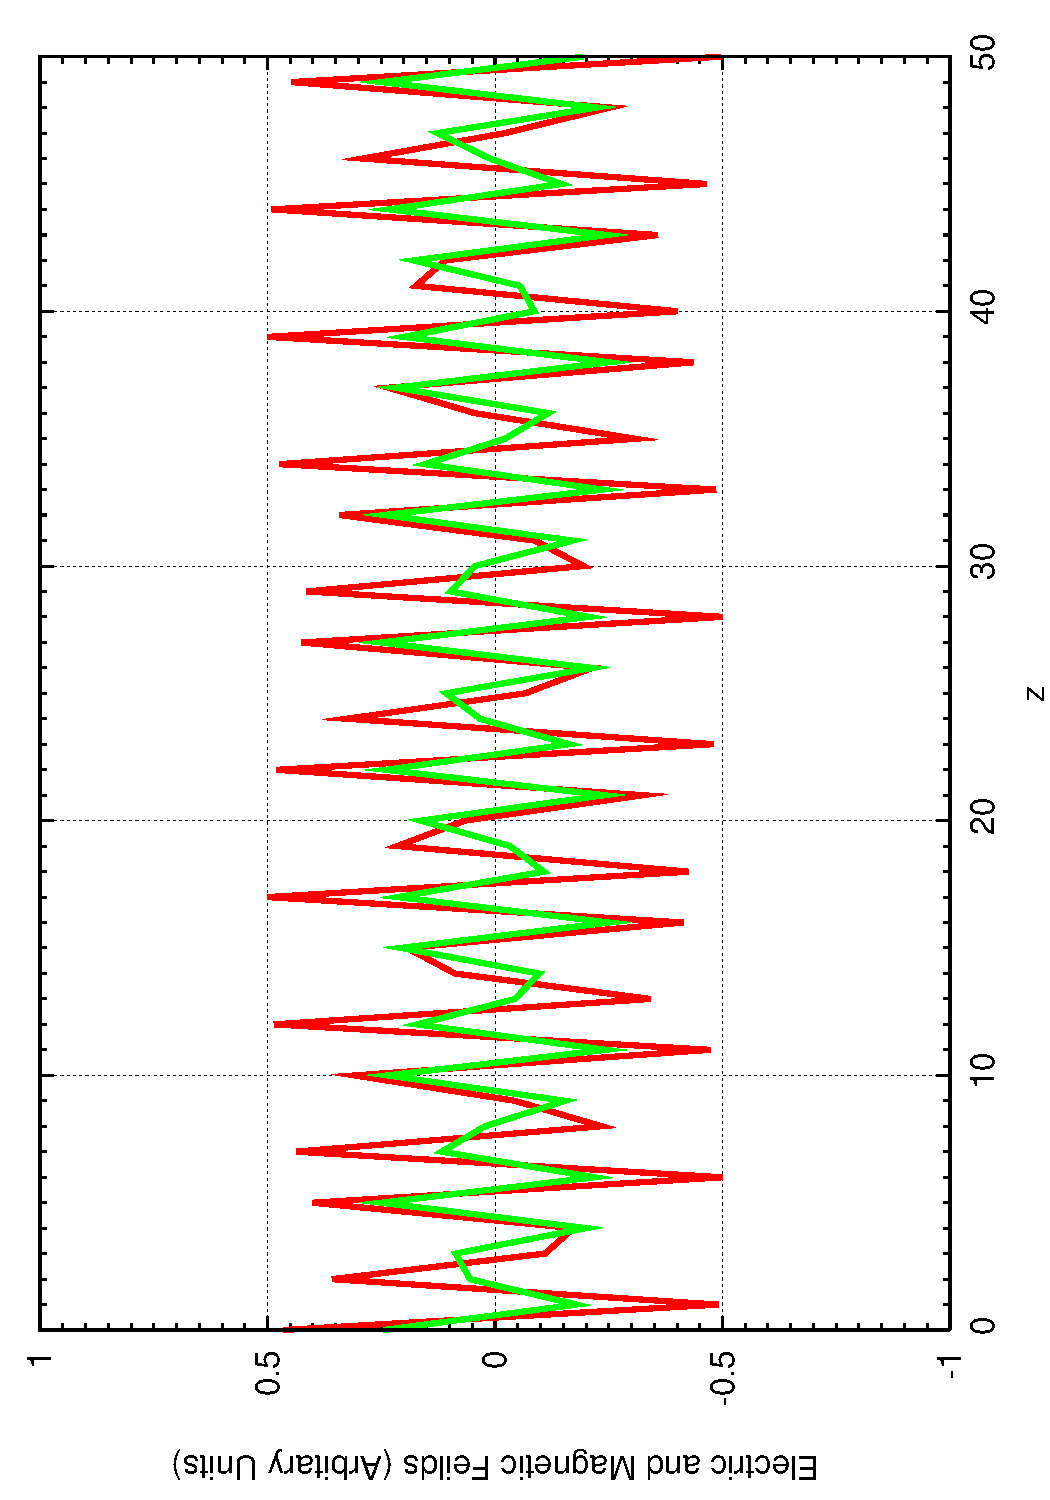
\includegraphics[angle=270, width=\textwidth]{highfreqsine4.pdf}
        \end{subfigure}
        \caption{The effect of aliasing on the accuracy of the function calculated by the simulation when plotting the function $0.5\sin(ax)$ for increasing $a$. The first two graphs show the wave at the usual resolution as used previously and the second two show the waves for higher frequencies with a shorter $x$ space so that the effect can be seen more clearly.}\label{fig:highfreqsine}
\end{figure}
The Fourier transform of a Gaussian represents the function in frequency space. For the function defined in equation~\ref{eq:gaussian}, the Fourier transform is $\mathcal{F}_x$. This is also a Gaussian function, as shown in figure~\ref{fig:fouriergauss}.
\begin{align}
        \mathcal{F}_x \left[\e{-ax^2}\right] (k) &= \int_{-\infty}^{\infty} \e{-ax^2}\e{-2\pi ikx}\D{x} \\
        &= \int_{-\infty}^{\infty} \e{-ax^2} \Big[\cos(2\pi kx)-i\sin(2\pi kx)\Big]\D{x} \\
        &= \int_{-\infty}^{\infty} \e{-ax^2} \cos(2\pi kx) dx -i\int_{-\infty}^{\infty}\sin(2\pi kx)\D{x} 
        \intertext{The second of these equations, $\int\sin(x)\D{x}$, is odd. Any odd function integrated over a symmetrical range is equal to 0, thus only the first integral makes a contribution.}
        \therefore \mathcal{F}_x\Big[\e{-ax^2}\Big](k) &= \sqrt{\frac{\pi}{a}}\e{\frac{-\pi^2 k^2}{a} }
\end{align} 
\begin{figure}[ht]
  \centering
  \begin{overpic}[angle=270, width=0.6\textwidth]{gaussian.pdf}
    \put(60,35){$\mathcal{F}_x(k) = \sqrt{\frac{\pi}{a}}\e{\frac{-\pi^2 k^2}{a} }$}
    \put(60,50){$f(x) = \e{-ax^2}$}
    \put(63,47){\vector(-3,-1){6}}
    \put(70,33){\vector(-3,-4){6}}
  \end{overpic}
  \caption{\label{fig:fouriergauss}The Fourier transform of the Gaussian function is also a Gaussian with a larger range of frequencies..}
\end{figure}

One of the effects of a dielectric is to separate out the frequencies in a travelling wave, since they move at different velocities in the material. This is the effect that is observed here. Since the Fourier transform shows that the frequencies are more widely spread, this happens to a greater degree the higher the frequency being modelled. 

This property means that unless the function is calculated to infinite precision, there will be some frequencies left out, and so not a perfect wave. This is the phenomenon that is taking place when the wave enters the dielectric material. When it enters the material, the wavelength gets shorter and so the frequency increases. This means that the high frequencies that make up the Gaussian function are also increased and since the simulation has a high temporal/spacial step, this causes the same aliasing as seen in figure~\ref{fig:highfreqsine}.

In order to correct this, or at least reduce its effect, the relative spacial/temporal step can be reduced. This means that there are more points calculated for the fields per unit length of the simulation area and so a greater accuracy of the results. When the spacial resolution is increased, there are naturally compromises in the time taken to calculate each frame. In figure~\ref{fig:highresolutuion1}, the size of the grid is changed from 200 nodes wide, to 2000 nodes wide. This has the effect of narrowing all of the function's appearance since they are all still calculated with optimisation of the previous width. Instead, the functions are changed so that they reflect the increase in width. This means that the function being plotted is in fact a different function, but since this represents only a scaling factor, and since the system has been scaled by the same factor, there is no difference in the observed behaviour.

\begin{figure}[ht]
        \centering
        \begin{subfigure}[ht]{0.45\textwidth}
                \centering
                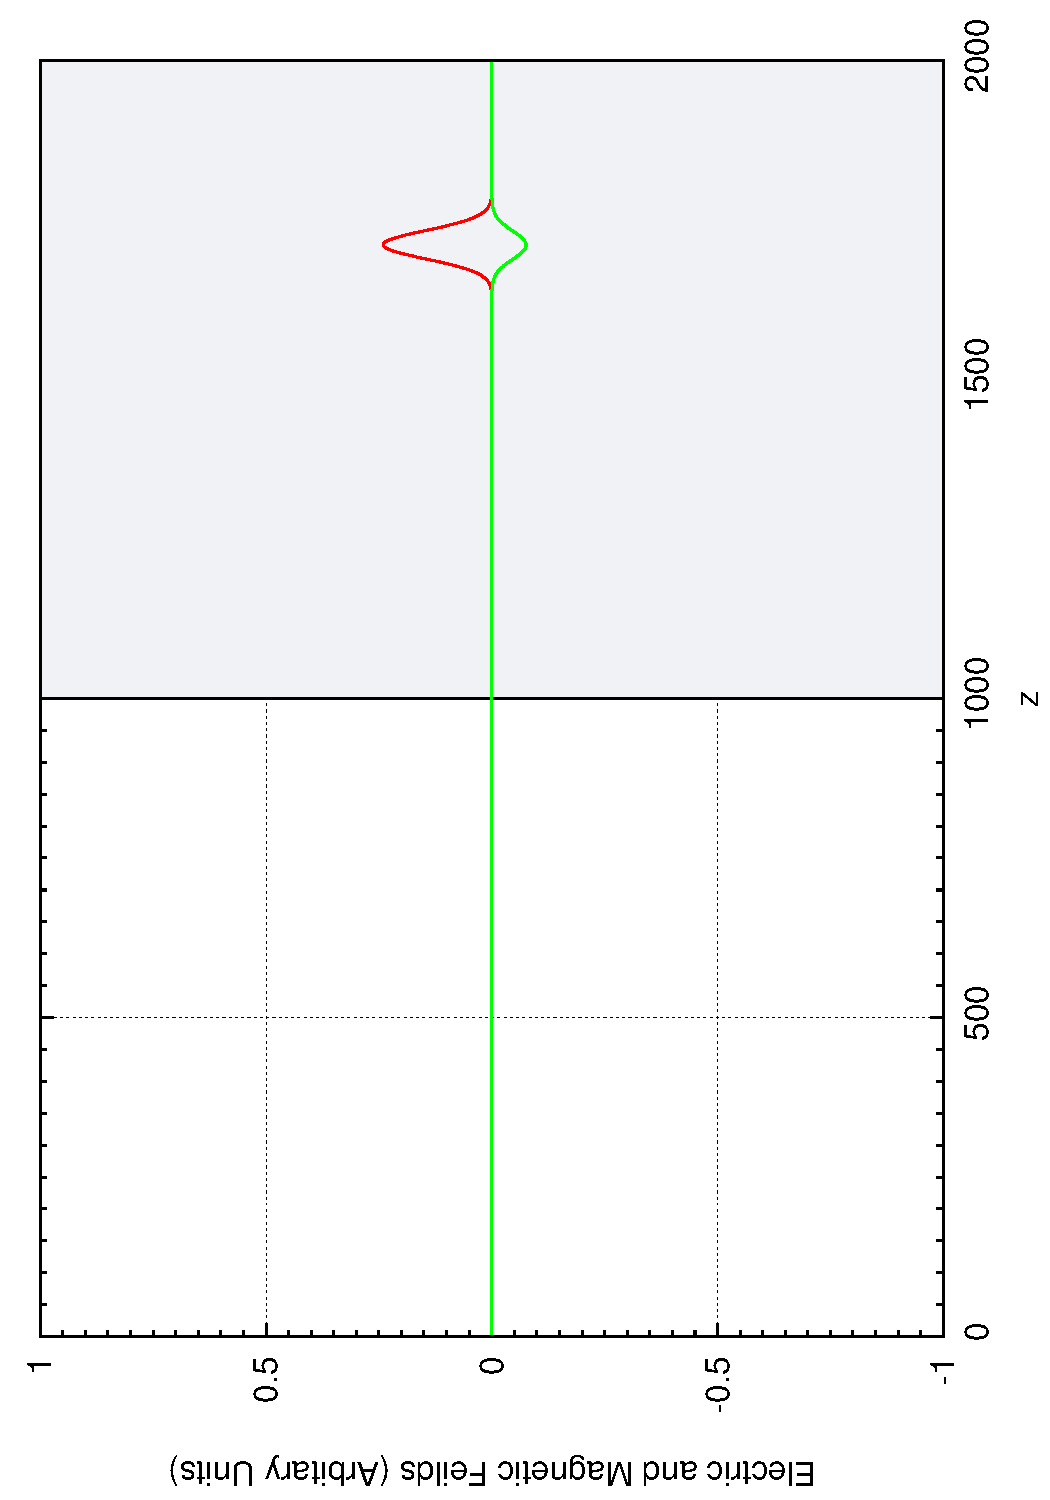
\includegraphics[angle=270, width=\textwidth]{gaussnoise2.pdf}
        \end{subfigure}%
        ~
        \begin{subfigure}[ht]{0.45\textwidth}
                \centering
                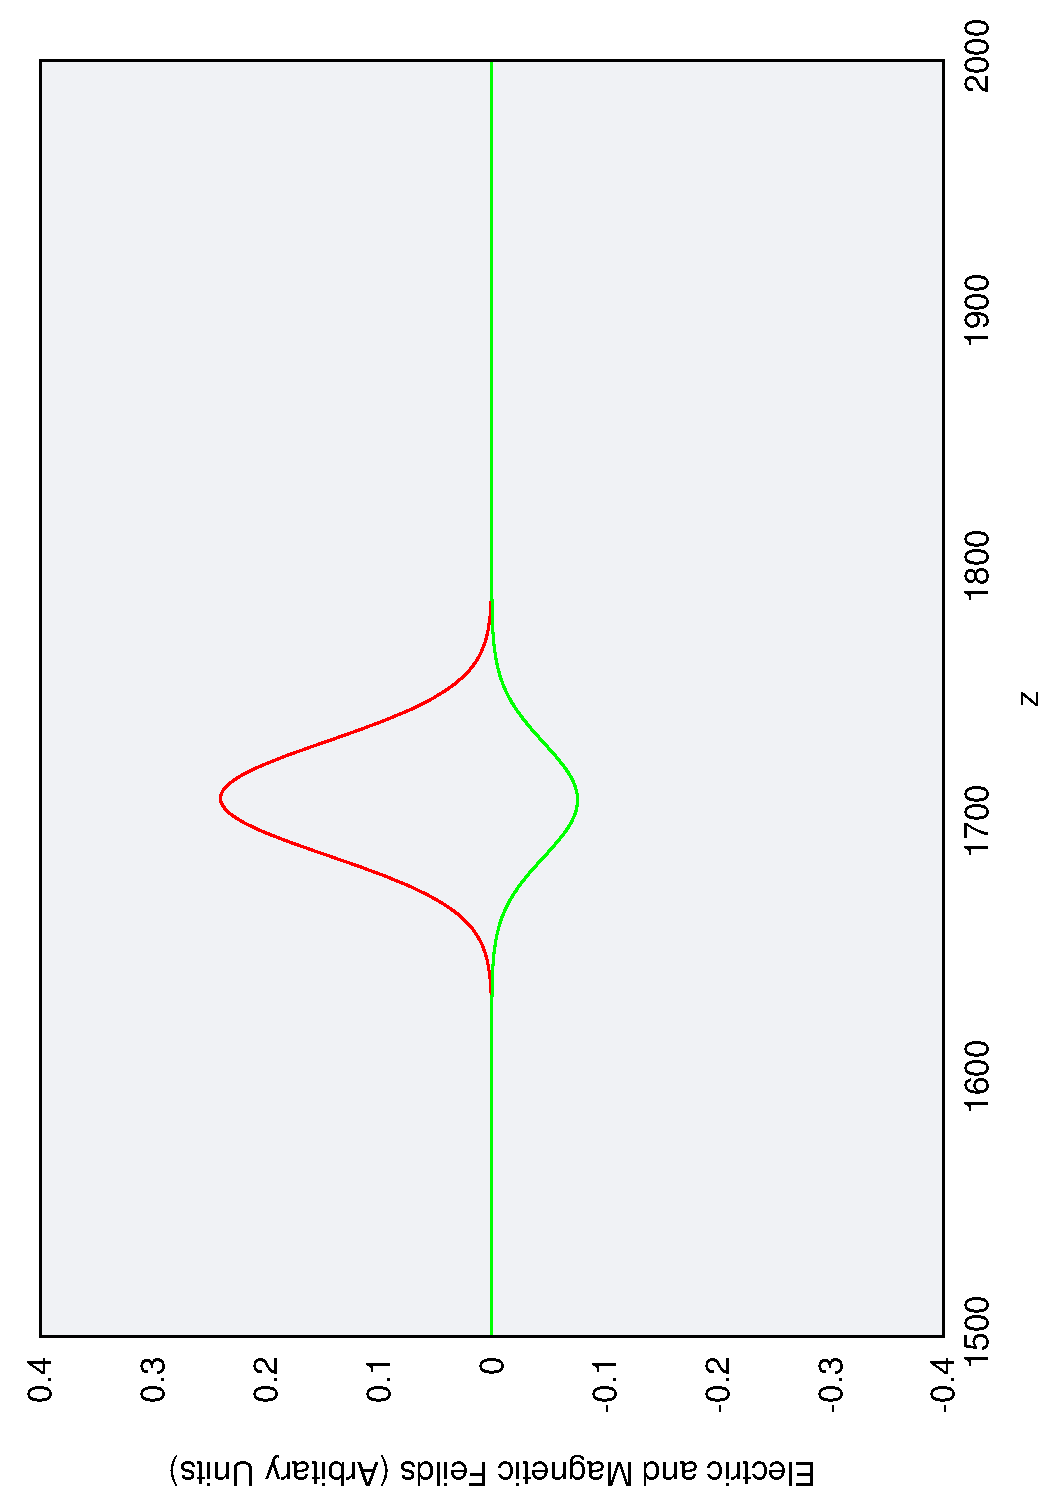
\includegraphics[angle=270, width=\textwidth]{gaussnoise2b.pdf}
        \end{subfigure}
        \caption{Two frames from a wave that is created in the centre of the region. The seed point creates two pulses that move away from each other. The amplitude is set to one half of previous so that when they interact after colliding with the walls, the resulting peak stays within the graphing area.}\label{fig:highresolutuion1}
\end{figure}
% subsubsection non_lossy_material (end)

\subsubsection{Lossy Material} % (fold)
\label{ssub:lossy_material}
A dielectric with a finite permittivity is simple to demonstrate since there is no change in the wave once it has entered the dielectric material. The only change to the wave is at the boundary, it is a homogeneous material. Instead, it is possible to add a loss factor to the dielectric so that the medium shows some inhomogeneity.

This is done by simply applying a scaling factor, or finite conductivity, on the wave which is dependant on the position in the dielectric as the wave moves through it. A conduction-current term can be added to the equation used to start with, equation~\ref{eq:max2}, as shown in equation~\ref{eq:conductioncurrent}.
\begin{align}
    \curl{\vec{H}} &= \epsilon \pd{\vec{E}}{t} + \sigma \vec{E}\label{eq:conductioncurrent} 
    \intertext{This can be reduced to the single dimension as before and written in terms of the variable part of the function}
    \dx{H_y}{x} &= \epsilon \dx{E_z}{t} + \sigma E_z
    \intertext{This equation can then be discretized for use with the FDTD algorithm so that the update equations become}
    \frac{H(m+\frac{1}{2})-H(m-\frac{1}{2})}{\delta} &= \epsilon \frac{E(m+1)-E(m)}{\delta} + \sigma \frac{E(m+1)+E(m)}{2}
\end{align}

The final term is the finite conductivity. This form is used as it is the time average of the electric field nodes at the points $m$ and $(m+1)$, since there is no node at the point $(m+\frac{1}{2})$.

When such a material is added to the simulation region, there is no change to the reflection coefficient, or the shape of the wave when first it enters the dielectric, compared to if the dielectric was not lossy. The only change that is observed is to the amplitude of the wave which slowly decreases as it moves through the material. Figure~\ref{fig:lossydiele} shows several stages of the wave as it is moving through the dielectric.

\begin{figure}[ht]
    \centering
    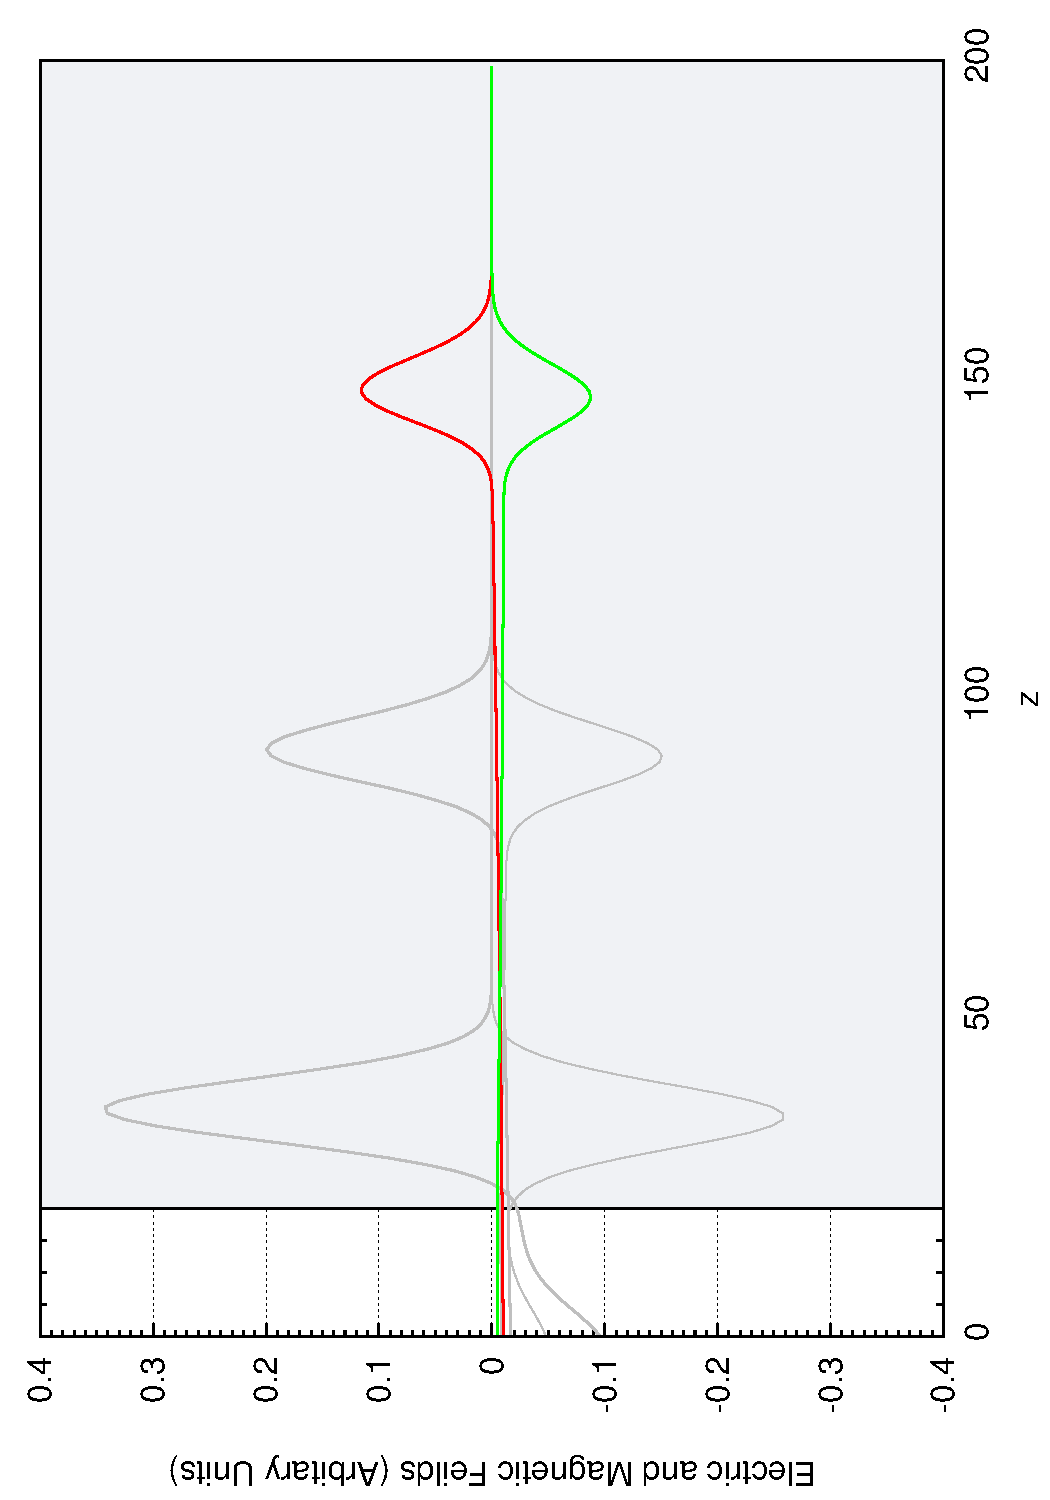
\includegraphics[angle=270, width=0.6\textwidth]{lossydielec1.pdf}
    \caption{Several frames showing the wave after it has entered the dielectric material. Each image is 80 frames apart. The lossyness of the dielectric has been set to 0.01 which means that each the amplitude of the wave is 99\% of its previous value for each step of the simulation .}\label{fig:lossydiele}
\end{figure}
% subsubsection lossy_material (end)
% subsection dielectirc_material (end)

\subsection{Total Field/Scattered Field Boundary} % (fold)
\label{sub:total_field_scattered_field_boundary}
So far, the only types of sources that have been modelled are the fixed and the additive source. These both result in a wave that is created at a single static point, and travels in both directions away from the source. But it is possible to initiate a wave such that it moves only in a single direction. We shall consider the case of a wave created and moving in the positive direction, from left to right, a very similar approach is needed for the opposite case. This is possible using a total field/scattered field boundary (TFSF). This is coded as simply the original field that is created moving in both directions, with an extra step that simply removes the magnitude of the wave from the direction that is not desired. 

So, for this example, a step that takes the Gaussian function away from the node on the left side of the source is added. This results in a wave that travels in only one direction. The TFSF method is similar to the total absorbing boundary we saw previously, that allowed the simulation area to be more than a confined box, but to extend to infinity. The difference here is that the wave is generated at this point, but if it were to be reflected back from a boundary and re-encounter this point, it would be able to travel through the source node as if it were any other node. An implementation  of the TFSF is shown in figure~\ref{fig:TFSF}, which also shows the same wave after it has been incident on a dielectric boundary and passed through the same source node again.

\begin{figure}[ht]
        \centering
        \begin{subfigure}[ht]{0.45\textwidth}
                \centering
                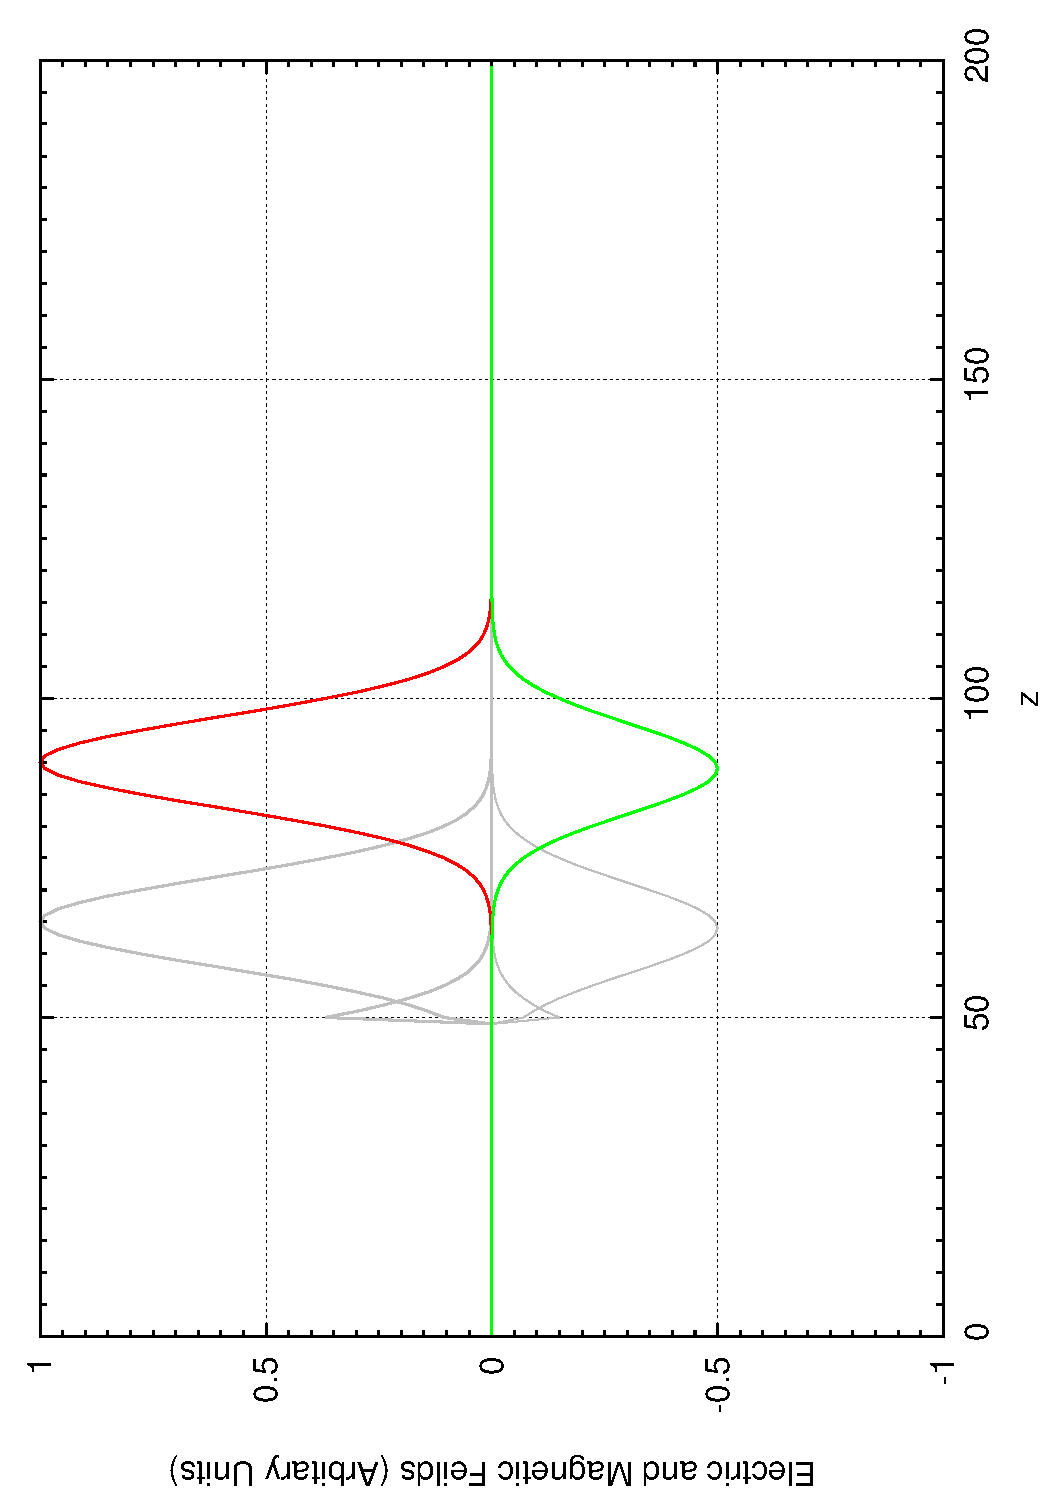
\includegraphics[angle=270, width=\textwidth]{TFSF1.pdf}
        \end{subfigure}%
        ~
        \begin{subfigure}[ht]{0.45\textwidth}
                \centering
                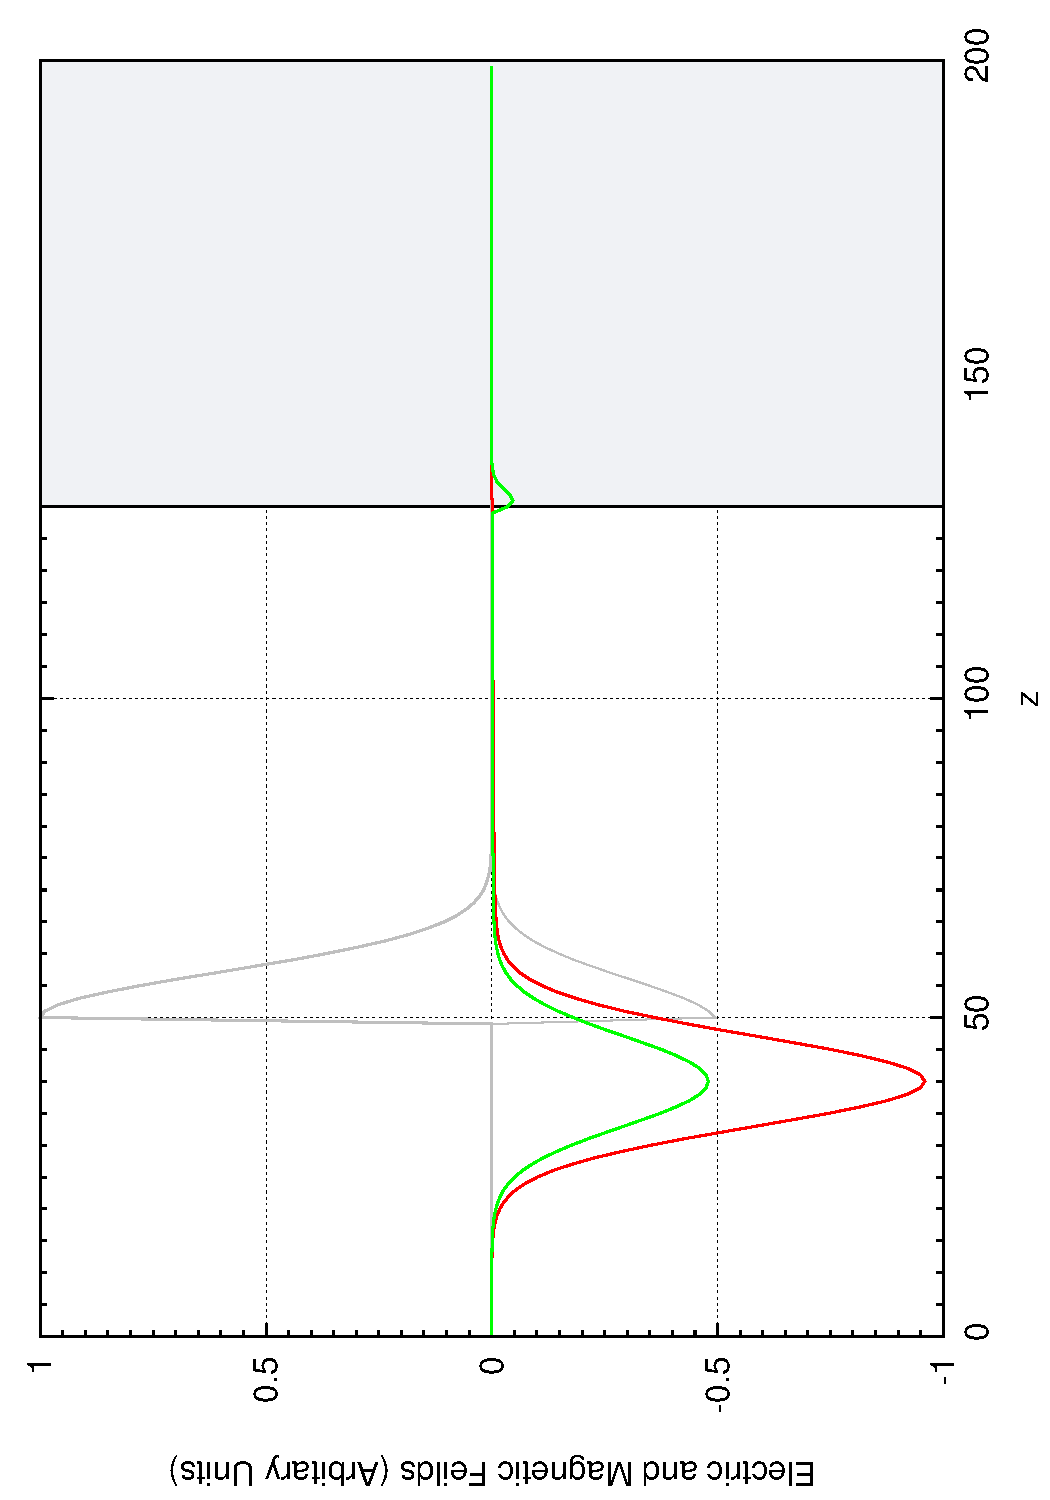
\includegraphics[angle=270, width=\textwidth]{TFSF2.pdf}
        \end{subfigure}
        \caption{Several frame showing the creation and resulting propagation of a wave created at a TFSF boundary, as well as a frame showing how the TFSF boundary acts like a regular node when the wave is reflected from a dielectric boundary and passes through the initial source point.}\label{fig:TFSF}
\end{figure}

The TFSF boundary gets its name from the resulting behaviour of the simulation area. Once a TFSF boundary is created, the area is separated into two distinct regions (again we shall consider only the case for the wave generated at the source and moving right). The right is the Total Field, the left is the Scattered Field. The source creates a wave that only exists in the total field initially, it is only if the wave encounters a boundary and scatters from it that it is able to reach the scattered field region.


% subsection total_field_scattered_field_boundary (end)

% section simulations (end)
